%
%  For more information, please see: http://software.sci.utah.edu
% 
%  The MIT License
% 
%  Copyright (c) 2004 Scientific Computing and Imaging Institute,
%  University of Utah.
% 
%  License for the specific language governing rights and limitations under
%  Permission is hereby granted, free of charge, to any person obtaining a
%  copy of this software and associated documentation files (the "Software"),
%  to deal in the Software without restriction, including without limitation
%  the rights to use, copy, modify, merge, publish, distribute, sublicense,
%  and/or sell copies of the Software, and to permit persons to whom the
%  Software is furnished to do so, subject to the following conditions:
% 
%  The above copyright notice and this permission notice shall be included
%  in all copies or substantial portions of the Software.
% 
%  THE SOFTWARE IS PROVIDED "AS IS", WITHOUT WARRANTY OF ANY KIND, EXPRESS
%  OR IMPLIED, INCLUDING BUT NOT LIMITED TO THE WARRANTIES OF MERCHANTABILITY,
%  FITNESS FOR A PARTICULAR PURPOSE AND NONINFRINGEMENT. IN NO EVENT SHALL
%  THE AUTHORS OR COPYRIGHT HOLDERS BE LIABLE FOR ANY CLAIM, DAMAGES OR OTHER
%  LIABILITY, WHETHER IN AN ACTION OF CONTRACT, TORT OR OTHERWISE, ARISING
%  FROM, OUT OF OR IN CONNECTION WITH THE SOFTWARE OR THE USE OR OTHER
%  DEALINGS IN THE SOFTWARE.
%


\documentclass[11pt,titlepage]{book}
\usepackage[]{html}
\usepackage[]{graphicx}
\usepackage[]{alltt}
\usepackage{makeidx}

\usepackage{scirun-doc}
% -*-latex-*-
%
%  The contents of this file are subject to the University of Utah Public
%  License (the "License"); you may not use this file except in compliance
%  with the License.
%
%  Software distributed under the License is distributed on an "AS IS"
%  basis, WITHOUT WARRANTY OF ANY KIND, either express or implied. See the
%  License for the specific language governing rights and limitations under
%  the License.
%
%  The Original Source Code is SCIRun, released March 12, 2001.
%
%  The Original Source Code was developed by the University of Utah.
%  Portions created by UNIVERSITY are Copyright (C) 2001, 1994
%  University of Utah. All Rights Reserved.
%

%
% Latex package to be used by scirun documents.  Markup commands exist
% in two files.  This one and scirun-doc.tex.  This file contains
% commands that are processed by both latex and by the builtin
% capabilities of latex2html.  Scirun-doc.sty contains commands that are
% either completely ignored by latex2html or are processed by functions in
% the latex2html extension file scirun-doc.perl.
%
% Documents should include the
% following latex commands:
%
% \usepackage{scirun-doc}
% % -*-latex-*-
%
%  The contents of this file are subject to the University of Utah Public
%  License (the "License"); you may not use this file except in compliance
%  with the License.
%
%  Software distributed under the License is distributed on an "AS IS"
%  basis, WITHOUT WARRANTY OF ANY KIND, either express or implied. See the
%  License for the specific language governing rights and limitations under
%  the License.
%
%  The Original Source Code is SCIRun, released March 12, 2001.
%
%  The Original Source Code was developed by the University of Utah.
%  Portions created by UNIVERSITY are Copyright (C) 2001, 1994
%  University of Utah. All Rights Reserved.
%

%
% Latex package to be used by scirun documents.  Markup commands exist
% in two files.  This one and scirun-doc.tex.  This file contains
% commands that are processed by both latex and by the builtin
% capabilities of latex2html.  Scirun-doc.sty contains commands that are
% either completely ignored by latex2html or are processed by functions in
% the latex2html extension file scirun-doc.perl.
%
% Documents should include the
% following latex commands:
%
% \usepackage{scirun-doc}
% % -*-latex-*-
%
%  The contents of this file are subject to the University of Utah Public
%  License (the "License"); you may not use this file except in compliance
%  with the License.
%
%  Software distributed under the License is distributed on an "AS IS"
%  basis, WITHOUT WARRANTY OF ANY KIND, either express or implied. See the
%  License for the specific language governing rights and limitations under
%  the License.
%
%  The Original Source Code is SCIRun, released March 12, 2001.
%
%  The Original Source Code was developed by the University of Utah.
%  Portions created by UNIVERSITY are Copyright (C) 2001, 1994
%  University of Utah. All Rights Reserved.
%

%
% Latex package to be used by scirun documents.  Markup commands exist
% in two files.  This one and scirun-doc.tex.  This file contains
% commands that are processed by both latex and by the builtin
% capabilities of latex2html.  Scirun-doc.sty contains commands that are
% either completely ignored by latex2html or are processed by functions in
% the latex2html extension file scirun-doc.perl.
%
% Documents should include the
% following latex commands:
%
% \usepackage{scirun-doc}
% \input{scirun-doc.tex}
%

% (Mostly) Short cuts  ==============================
\newcommand{\SCI}{{\em SCI}}
\newcommand{\sci}{\SCI}
\newcommand{\scii}{SCI Institute}
\newcommand{\BIOPSE}{\textbf{BioPSE}}
\newcommand{\biopse}{\BIOPSE}
\newcommand{\SR}{\textbf{SCIRun}}
\newcommand{\sr}{\SR}
\newcommand{\eg}{{\em e.g.,}}
\newcommand{\ie}{{\em i.e.,}}
\newcommand{\etc}{{\em etc.}}
\newcommand{\etal}{{\em et al.}}
\newcommand{\degrees}{{$^{\circ}$}}
\newcommand{\splitline}{\begin{center}\rule{\columnwidth}{.7mm}\end{center}}
\newcommand{\X}[1]{#1\index{#1}}
\newcommand{\srig}{\sr{} Installation Guide}
\newcommand{\srug}{\sr{} User's Guide}
\newcommand{\srdg}{\sr{} Developer's Guide}

% Literal ~ character
\newcommand{\ltilde}{\textasciitilde}

% Encloses its argument between angle brackets.
\newcommand{\ab}[1]{\textless{}#1\textgreater}

% Inserts a left angle bracket.
\newcommand{\la}{\textless}

% Inserts a right angle bracket.
\newcommand{\ra}{\textgreater}


% Mark up commands =================================

% Url
%\newcommand{\url}[1]{#1}

% ip address
\newcommand{\ipaddr}[1]{#1}
\newcommand{\localhost}{\ipaddr{127.0.0.1}}

% Predefined acronyms
\newcommand{\gui}{\acronym{GUI}}
\newcommand{\tcl}{\acronym{TCL}}
\newcommand{\xml}{\acronym{XML}}
\newcommand{\pse}{\acronym{PSE}}

% Markup the first time use of term that may be unfamiliar to the
% reader. 
\newmucmd{dfn}{emph}

% In the next command #1 is the term and #2 is the shortcut or acronym that
% will be used in the rest of the document. 
\newcommand{\dfna}[2]{\emph{#1} (\acronym{#2})}

% Markup a file name.
\newmucmd{filename}{texttt}

% Directory name markup.
\newmucmd{directory}{texttt}

% Markup text which is the name of a command.
\newmucmd{command}{texttt} 

% Command option.
\newmucmd{option}{texttt}

% Markup text typed at the keyboard.
\newmucmd{keyboard}{texttt} 

% Parameterized text - marks up text that is to be
% substituted for by the reader.
\newmucmd{ptext}{textit}        % Obsolete-use replaceable instead.
\newmucmd{replaceable}{textit}

% Markup text the user might see on his screen.
\newmucmd{screen}{texttt}

% Markup the name of a GUI menu.
\newmucmd{guimenu}{textbf}

% Markup the name of a GUI menu.
\newcommand{\menu}[1]{\guimenu{#1}}

% Markup a gui menu item name.
\newmucmd{guimenuitem}{textbf}

% Markup a menu item name.
\newcommand{\menuitem}[1]{\guimenuitem{#1}}

% Markup name of a ui button.
\newmucmd{guibutton}{textbf}

% Markup name of a ui button.
\newcommand{\button}[1]{\guibutton{#1}}

% Markup name of a gui text item.
\newmucmd{guitext}{textit}

% Markup name of a gui label.
\newmucmd{guilabel}{textbf}

% GUI variable
\newmucmd{guivar}{texttt}

% Scirun port
\newmucmd{srport}{texttt}

% Sockets port
\newcommand{\port}[1]{\texttt{#1}}

% Socket
\newcommand{\socket}[2]{\texttt{#1:#2}}

% Variable
\newcommand{\variable}[1]{\texttt{#1}}

% Data type
\newcommand{\datatype}[1]{\texttt{#1}}

% Function
\newcommand{\function}[1]{\texttt{#1}}

% Markup an inline code fragment.
\newcommand{\icode}[1]{\texttt{#1}}

% Markup a module name.
\newcommand{\module}[1]{\texttt{#1}}

% Markup a sr package name.
\newcommand{\package}[1]{\texttt{#1}}

% Markup a sr category name.
\newcommand{\category}[1]{\texttt{#1}}

% Env variable markup.
\newmucmd{envvar}{texttt}

% Markup for the title of a book or article or whatever.
\newcommand{\etitle}[1]{\texttt{#1}}

% Markup name of a latex section.  First arg is section name.  Second arg
% is section's label.  When processed with latex, the section
% name is emphasized.  When processed with latex2html section name is made
% into a link to section.
\newcommand{\secname}[2]{\latexhtml{\emph{#1}}{\htmlref{#1}{#2}}}

% Section ref command.  Use of this command
% in place of \ref to reference sections (subsections etc.) will
% create a more web friendly version of your document.
% The command's first argument is the link text (used only on the html
% page) and the second argument is the section's label
\newcommand{\secref}[2]{\hyperref[ref]{\emph{#1}}{Section~}{}{#2}}
\newcommand{\chref}[2]{\hyperref[ref]{\emph{#1}}{Chapter~}{}{#2}}

% A latex command
\newcommand{\latexcommand}[1]{\texttt{\textbackslash#1}}

% A latex package
\newcommand{\latexpackage}[1]{\textit{#1}}

% Use these in place of missing content.
\newcommand{\missing}[1]{\emph{#1 - Coming Soon.}}

% Use this to make note of incomplete content.
\newcommand{\incomplete}{\emph{More Comming Soon.}}

% Mark up a mail address
\newmucmd{mailto}{texttt}

% Mark up an xml attribute
\newmucmd{xmlattrname}{texttt}

% Sci Urls ========================================= 

% www style urls.
\newcommand{\scisoftware}{http://software.sci.utah.edu}
\newcommand{\scisoftwareurl}{\scisoftware}
\newcommand{\sciurl}{http://www.sci.utah.edu}
\newcommand{\scidocurl}{\scisoftware{}/doc}
\newcommand{\scidocurlplus}[1]{\scisoftware{}/doc/#1}
\newcommand{\bugsurl}{\scisoftware{}/bugzilla}
\newcommand{\scisoftwarearchiveurl}{\scisoftware{}/archive\_entry.html}

%

% (Mostly) Short cuts  ==============================
\newcommand{\SCI}{{\em SCI}}
\newcommand{\sci}{\SCI}
\newcommand{\scii}{SCI Institute}
\newcommand{\BIOPSE}{\textbf{BioPSE}}
\newcommand{\biopse}{\BIOPSE}
\newcommand{\SR}{\textbf{SCIRun}}
\newcommand{\sr}{\SR}
\newcommand{\eg}{{\em e.g.,}}
\newcommand{\ie}{{\em i.e.,}}
\newcommand{\etc}{{\em etc.}}
\newcommand{\etal}{{\em et al.}}
\newcommand{\degrees}{{$^{\circ}$}}
\newcommand{\splitline}{\begin{center}\rule{\columnwidth}{.7mm}\end{center}}
\newcommand{\X}[1]{#1\index{#1}}
\newcommand{\srig}{\sr{} Installation Guide}
\newcommand{\srug}{\sr{} User's Guide}
\newcommand{\srdg}{\sr{} Developer's Guide}

% Literal ~ character
\newcommand{\ltilde}{\textasciitilde}

% Encloses its argument between angle brackets.
\newcommand{\ab}[1]{\textless{}#1\textgreater}

% Inserts a left angle bracket.
\newcommand{\la}{\textless}

% Inserts a right angle bracket.
\newcommand{\ra}{\textgreater}


% Mark up commands =================================

% Url
%\newcommand{\url}[1]{#1}

% ip address
\newcommand{\ipaddr}[1]{#1}
\newcommand{\localhost}{\ipaddr{127.0.0.1}}

% Predefined acronyms
\newcommand{\gui}{\acronym{GUI}}
\newcommand{\tcl}{\acronym{TCL}}
\newcommand{\xml}{\acronym{XML}}
\newcommand{\pse}{\acronym{PSE}}

% Markup the first time use of term that may be unfamiliar to the
% reader. 
\newmucmd{dfn}{emph}

% In the next command #1 is the term and #2 is the shortcut or acronym that
% will be used in the rest of the document. 
\newcommand{\dfna}[2]{\emph{#1} (\acronym{#2})}

% Markup a file name.
\newmucmd{filename}{texttt}

% Directory name markup.
\newmucmd{directory}{texttt}

% Markup text which is the name of a command.
\newmucmd{command}{texttt} 

% Command option.
\newmucmd{option}{texttt}

% Markup text typed at the keyboard.
\newmucmd{keyboard}{texttt} 

% Parameterized text - marks up text that is to be
% substituted for by the reader.
\newmucmd{ptext}{textit}        % Obsolete-use replaceable instead.
\newmucmd{replaceable}{textit}

% Markup text the user might see on his screen.
\newmucmd{screen}{texttt}

% Markup the name of a GUI menu.
\newmucmd{guimenu}{textbf}

% Markup the name of a GUI menu.
\newcommand{\menu}[1]{\guimenu{#1}}

% Markup a gui menu item name.
\newmucmd{guimenuitem}{textbf}

% Markup a menu item name.
\newcommand{\menuitem}[1]{\guimenuitem{#1}}

% Markup name of a ui button.
\newmucmd{guibutton}{textbf}

% Markup name of a ui button.
\newcommand{\button}[1]{\guibutton{#1}}

% Markup name of a gui text item.
\newmucmd{guitext}{textit}

% Markup name of a gui label.
\newmucmd{guilabel}{textbf}

% GUI variable
\newmucmd{guivar}{texttt}

% Scirun port
\newmucmd{srport}{texttt}

% Sockets port
\newcommand{\port}[1]{\texttt{#1}}

% Socket
\newcommand{\socket}[2]{\texttt{#1:#2}}

% Variable
\newcommand{\variable}[1]{\texttt{#1}}

% Data type
\newcommand{\datatype}[1]{\texttt{#1}}

% Function
\newcommand{\function}[1]{\texttt{#1}}

% Markup an inline code fragment.
\newcommand{\icode}[1]{\texttt{#1}}

% Markup a module name.
\newcommand{\module}[1]{\texttt{#1}}

% Markup a sr package name.
\newcommand{\package}[1]{\texttt{#1}}

% Markup a sr category name.
\newcommand{\category}[1]{\texttt{#1}}

% Env variable markup.
\newmucmd{envvar}{texttt}

% Markup for the title of a book or article or whatever.
\newcommand{\etitle}[1]{\texttt{#1}}

% Markup name of a latex section.  First arg is section name.  Second arg
% is section's label.  When processed with latex, the section
% name is emphasized.  When processed with latex2html section name is made
% into a link to section.
\newcommand{\secname}[2]{\latexhtml{\emph{#1}}{\htmlref{#1}{#2}}}

% Section ref command.  Use of this command
% in place of \ref to reference sections (subsections etc.) will
% create a more web friendly version of your document.
% The command's first argument is the link text (used only on the html
% page) and the second argument is the section's label
\newcommand{\secref}[2]{\hyperref[ref]{\emph{#1}}{Section~}{}{#2}}
\newcommand{\chref}[2]{\hyperref[ref]{\emph{#1}}{Chapter~}{}{#2}}

% A latex command
\newcommand{\latexcommand}[1]{\texttt{\textbackslash#1}}

% A latex package
\newcommand{\latexpackage}[1]{\textit{#1}}

% Use these in place of missing content.
\newcommand{\missing}[1]{\emph{#1 - Coming Soon.}}

% Use this to make note of incomplete content.
\newcommand{\incomplete}{\emph{More Comming Soon.}}

% Mark up a mail address
\newmucmd{mailto}{texttt}

% Mark up an xml attribute
\newmucmd{xmlattrname}{texttt}

% Sci Urls ========================================= 

% www style urls.
\newcommand{\scisoftware}{http://software.sci.utah.edu}
\newcommand{\scisoftwareurl}{\scisoftware}
\newcommand{\sciurl}{http://www.sci.utah.edu}
\newcommand{\scidocurl}{\scisoftware{}/doc}
\newcommand{\scidocurlplus}[1]{\scisoftware{}/doc/#1}
\newcommand{\bugsurl}{\scisoftware{}/bugzilla}
\newcommand{\scisoftwarearchiveurl}{\scisoftware{}/archive\_entry.html}

%

% (Mostly) Short cuts  ==============================
\newcommand{\SCI}{{\em SCI}}
\newcommand{\sci}{\SCI}
\newcommand{\scii}{SCI Institute}
\newcommand{\BIOPSE}{\textbf{BioPSE}}
\newcommand{\biopse}{\BIOPSE}
\newcommand{\SR}{\textbf{SCIRun}}
\newcommand{\sr}{\SR}
\newcommand{\eg}{{\em e.g.,}}
\newcommand{\ie}{{\em i.e.,}}
\newcommand{\etc}{{\em etc.}}
\newcommand{\etal}{{\em et al.}}
\newcommand{\degrees}{{$^{\circ}$}}
\newcommand{\splitline}{\begin{center}\rule{\columnwidth}{.7mm}\end{center}}
\newcommand{\X}[1]{#1\index{#1}}
\newcommand{\srig}{\sr{} Installation Guide}
\newcommand{\srug}{\sr{} User's Guide}
\newcommand{\srdg}{\sr{} Developer's Guide}

% Literal ~ character
\newcommand{\ltilde}{\textasciitilde}

% Encloses its argument between angle brackets.
\newcommand{\ab}[1]{\textless{}#1\textgreater}

% Inserts a left angle bracket.
\newcommand{\la}{\textless}

% Inserts a right angle bracket.
\newcommand{\ra}{\textgreater}


% Mark up commands =================================

% Url
%\newcommand{\url}[1]{#1}

% ip address
\newcommand{\ipaddr}[1]{#1}
\newcommand{\localhost}{\ipaddr{127.0.0.1}}

% Predefined acronyms
\newcommand{\gui}{\acronym{GUI}}
\newcommand{\tcl}{\acronym{TCL}}
\newcommand{\xml}{\acronym{XML}}
\newcommand{\pse}{\acronym{PSE}}

% Markup the first time use of term that may be unfamiliar to the
% reader. 
\newmucmd{dfn}{emph}

% In the next command #1 is the term and #2 is the shortcut or acronym that
% will be used in the rest of the document. 
\newcommand{\dfna}[2]{\emph{#1} (\acronym{#2})}

% Markup a file name.
\newmucmd{filename}{texttt}

% Directory name markup.
\newmucmd{directory}{texttt}

% Markup text which is the name of a command.
\newmucmd{command}{texttt} 

% Command option.
\newmucmd{option}{texttt}

% Markup text typed at the keyboard.
\newmucmd{keyboard}{texttt} 

% Parameterized text - marks up text that is to be
% substituted for by the reader.
\newmucmd{ptext}{textit}        % Obsolete-use replaceable instead.
\newmucmd{replaceable}{textit}

% Markup text the user might see on his screen.
\newmucmd{screen}{texttt}

% Markup the name of a GUI menu.
\newmucmd{guimenu}{textbf}

% Markup the name of a GUI menu.
\newcommand{\menu}[1]{\guimenu{#1}}

% Markup a gui menu item name.
\newmucmd{guimenuitem}{textbf}

% Markup a menu item name.
\newcommand{\menuitem}[1]{\guimenuitem{#1}}

% Markup name of a ui button.
\newmucmd{guibutton}{textbf}

% Markup name of a ui button.
\newcommand{\button}[1]{\guibutton{#1}}

% Markup name of a gui text item.
\newmucmd{guitext}{textit}

% Markup name of a gui label.
\newmucmd{guilabel}{textbf}

% GUI variable
\newmucmd{guivar}{texttt}

% Scirun port
\newmucmd{srport}{texttt}

% Sockets port
\newcommand{\port}[1]{\texttt{#1}}

% Socket
\newcommand{\socket}[2]{\texttt{#1:#2}}

% Variable
\newcommand{\variable}[1]{\texttt{#1}}

% Data type
\newcommand{\datatype}[1]{\texttt{#1}}

% Function
\newcommand{\function}[1]{\texttt{#1}}

% Markup an inline code fragment.
\newcommand{\icode}[1]{\texttt{#1}}

% Markup a module name.
\newcommand{\module}[1]{\texttt{#1}}

% Markup a sr package name.
\newcommand{\package}[1]{\texttt{#1}}

% Markup a sr category name.
\newcommand{\category}[1]{\texttt{#1}}

% Env variable markup.
\newmucmd{envvar}{texttt}

% Markup for the title of a book or article or whatever.
\newcommand{\etitle}[1]{\texttt{#1}}

% Markup name of a latex section.  First arg is section name.  Second arg
% is section's label.  When processed with latex, the section
% name is emphasized.  When processed with latex2html section name is made
% into a link to section.
\newcommand{\secname}[2]{\latexhtml{\emph{#1}}{\htmlref{#1}{#2}}}

% Section ref command.  Use of this command
% in place of \ref to reference sections (subsections etc.) will
% create a more web friendly version of your document.
% The command's first argument is the link text (used only on the html
% page) and the second argument is the section's label
\newcommand{\secref}[2]{\hyperref[ref]{\emph{#1}}{Section~}{}{#2}}
\newcommand{\chref}[2]{\hyperref[ref]{\emph{#1}}{Chapter~}{}{#2}}

% A latex command
\newcommand{\latexcommand}[1]{\texttt{\textbackslash#1}}

% A latex package
\newcommand{\latexpackage}[1]{\textit{#1}}

% Use these in place of missing content.
\newcommand{\missing}[1]{\emph{#1 - Coming Soon.}}

% Use this to make note of incomplete content.
\newcommand{\incomplete}{\emph{More Comming Soon.}}

% Mark up a mail address
\newmucmd{mailto}{texttt}

% Mark up an xml attribute
\newmucmd{xmlattrname}{texttt}

% Sci Urls ========================================= 

% www style urls.
\newcommand{\scisoftware}{http://software.sci.utah.edu}
\newcommand{\scisoftwareurl}{\scisoftware}
\newcommand{\sciurl}{http://www.sci.utah.edu}
\newcommand{\scidocurl}{\scisoftware{}/doc}
\newcommand{\scidocurlplus}[1]{\scisoftware{}/doc/#1}
\newcommand{\bugsurl}{\scisoftware{}/bugzilla}
\newcommand{\scisoftwarearchiveurl}{\scisoftware{}/archive\_entry.html}

% -*-latex-*-
%
%  The contents of this file are subject to the University of Utah Public
%  License (the "License"); you may not use this file except in compliance
%  with the License.
%
%  Software distributed under the License is distributed on an "AS IS"
%  basis, WITHOUT WARRANTY OF ANY KIND, either express or implied. See the
%  License for the specific language governing rights and limitations under
%  the License.
%
%  The Original Source Code is SCIRun, released March 12, 2001.
%
%  The Original Source Code was developed by the University of Utah.
%  Portions created by UNIVERSITY are Copyright (C) 2001, 1994
%  University of Utah. All Rights Reserved.
%
% Markup and style for SCIRun Users guide.
%
\textheight 9.5in
\textwidth 7in
\topmargin -.50in
\oddsidemargin -.25in
\sloppy

% Fancy headings stuff
\pagestyle{fancy}
\headsep .08in
\footskip 25pt
\headheight 15pt
\setlength{\footrulewidth}{.8pt}
%\setlength{\headrulewidth}{.8pt}
\rhead{{ \PSE{} Users' Manual}}
\lhead{Version \version}
\lfoot{}
\cfoot{}
\rfoot{{\small \sf Page: \hspace{1em}\thepage\hspace{1em}}}

% Setting to control figure placement.
% These determine the rules used to place floating objects like figures 
% They are only guides, but read the manual to see the effect of each.
\renewcommand{\topfraction}{.8}
\renewcommand{\bottomfraction}{.8}
\renewcommand{\textfraction}{.1}

% Paragraph spacing
% This sets the spacing between paragraphs
\setlength{\parskip}{\smallskipamount} 

% Common markup commands
% -*-latex-*-
%
%  The contents of this file are subject to the University of Utah Public
%  License (the "License"); you may not use this file except in compliance
%  with the License.
%
%  Software distributed under the License is distributed on an "AS IS"
%  basis, WITHOUT WARRANTY OF ANY KIND, either express or implied. See the
%  License for the specific language governing rights and limitations under
%  the License.
%
%  The Original Source Code is SCIRun, released March 12, 2001.
%
%  The Original Source Code was developed by the University of Utah.
%  Portions created by UNIVERSITY are Copyright (C) 2001, 1994
%  University of Utah. All Rights Reserved.
%

%
% Latex package to be used by scirun documents.  Markup commands exist
% in two files.  This one and scirun-doc.tex.  This file contains
% commands that are processed by both latex and by the builtin
% capabilities of latex2html.  Scirun-doc.sty contains commands that are
% either completely ignored by latex2html or are processed by functions in
% the latex2html extension file scirun-doc.perl.
%
% Documents should include the
% following latex commands:
%
% \usepackage{scirun-doc}
% % -*-latex-*-
%
%  The contents of this file are subject to the University of Utah Public
%  License (the "License"); you may not use this file except in compliance
%  with the License.
%
%  Software distributed under the License is distributed on an "AS IS"
%  basis, WITHOUT WARRANTY OF ANY KIND, either express or implied. See the
%  License for the specific language governing rights and limitations under
%  the License.
%
%  The Original Source Code is SCIRun, released March 12, 2001.
%
%  The Original Source Code was developed by the University of Utah.
%  Portions created by UNIVERSITY are Copyright (C) 2001, 1994
%  University of Utah. All Rights Reserved.
%

%
% Latex package to be used by scirun documents.  Markup commands exist
% in two files.  This one and scirun-doc.tex.  This file contains
% commands that are processed by both latex and by the builtin
% capabilities of latex2html.  Scirun-doc.sty contains commands that are
% either completely ignored by latex2html or are processed by functions in
% the latex2html extension file scirun-doc.perl.
%
% Documents should include the
% following latex commands:
%
% \usepackage{scirun-doc}
% \input{scirun-doc.tex}
%

% (Mostly) Short cuts  ==============================
\newcommand{\SCI}{{\em SCI}}
\newcommand{\sci}{\SCI}
\newcommand{\scii}{SCI Institute}
\newcommand{\BIOPSE}{\textbf{BioPSE}}
\newcommand{\biopse}{\BIOPSE}
\newcommand{\SR}{\textbf{SCIRun}}
\newcommand{\sr}{\SR}
\newcommand{\eg}{{\em e.g.,}}
\newcommand{\ie}{{\em i.e.,}}
\newcommand{\etc}{{\em etc.}}
\newcommand{\etal}{{\em et al.}}
\newcommand{\degrees}{{$^{\circ}$}}
\newcommand{\splitline}{\begin{center}\rule{\columnwidth}{.7mm}\end{center}}
\newcommand{\X}[1]{#1\index{#1}}
\newcommand{\srig}{\sr{} Installation Guide}
\newcommand{\srug}{\sr{} User's Guide}
\newcommand{\srdg}{\sr{} Developer's Guide}

% Literal ~ character
\newcommand{\ltilde}{\textasciitilde}

% Encloses its argument between angle brackets.
\newcommand{\ab}[1]{\textless{}#1\textgreater}

% Inserts a left angle bracket.
\newcommand{\la}{\textless}

% Inserts a right angle bracket.
\newcommand{\ra}{\textgreater}


% Mark up commands =================================

% Url
%\newcommand{\url}[1]{#1}

% ip address
\newcommand{\ipaddr}[1]{#1}
\newcommand{\localhost}{\ipaddr{127.0.0.1}}

% Predefined acronyms
\newcommand{\gui}{\acronym{GUI}}
\newcommand{\tcl}{\acronym{TCL}}
\newcommand{\xml}{\acronym{XML}}
\newcommand{\pse}{\acronym{PSE}}

% Markup the first time use of term that may be unfamiliar to the
% reader. 
\newmucmd{dfn}{emph}

% In the next command #1 is the term and #2 is the shortcut or acronym that
% will be used in the rest of the document. 
\newcommand{\dfna}[2]{\emph{#1} (\acronym{#2})}

% Markup a file name.
\newmucmd{filename}{texttt}

% Directory name markup.
\newmucmd{directory}{texttt}

% Markup text which is the name of a command.
\newmucmd{command}{texttt} 

% Command option.
\newmucmd{option}{texttt}

% Markup text typed at the keyboard.
\newmucmd{keyboard}{texttt} 

% Parameterized text - marks up text that is to be
% substituted for by the reader.
\newmucmd{ptext}{textit}        % Obsolete-use replaceable instead.
\newmucmd{replaceable}{textit}

% Markup text the user might see on his screen.
\newmucmd{screen}{texttt}

% Markup the name of a GUI menu.
\newmucmd{guimenu}{textbf}

% Markup the name of a GUI menu.
\newcommand{\menu}[1]{\guimenu{#1}}

% Markup a gui menu item name.
\newmucmd{guimenuitem}{textbf}

% Markup a menu item name.
\newcommand{\menuitem}[1]{\guimenuitem{#1}}

% Markup name of a ui button.
\newmucmd{guibutton}{textbf}

% Markup name of a ui button.
\newcommand{\button}[1]{\guibutton{#1}}

% Markup name of a gui text item.
\newmucmd{guitext}{textit}

% Markup name of a gui label.
\newmucmd{guilabel}{textbf}

% GUI variable
\newmucmd{guivar}{texttt}

% Scirun port
\newmucmd{srport}{texttt}

% Sockets port
\newcommand{\port}[1]{\texttt{#1}}

% Socket
\newcommand{\socket}[2]{\texttt{#1:#2}}

% Variable
\newcommand{\variable}[1]{\texttt{#1}}

% Data type
\newcommand{\datatype}[1]{\texttt{#1}}

% Function
\newcommand{\function}[1]{\texttt{#1}}

% Markup an inline code fragment.
\newcommand{\icode}[1]{\texttt{#1}}

% Markup a module name.
\newcommand{\module}[1]{\texttt{#1}}

% Markup a sr package name.
\newcommand{\package}[1]{\texttt{#1}}

% Markup a sr category name.
\newcommand{\category}[1]{\texttt{#1}}

% Env variable markup.
\newmucmd{envvar}{texttt}

% Markup for the title of a book or article or whatever.
\newcommand{\etitle}[1]{\texttt{#1}}

% Markup name of a latex section.  First arg is section name.  Second arg
% is section's label.  When processed with latex, the section
% name is emphasized.  When processed with latex2html section name is made
% into a link to section.
\newcommand{\secname}[2]{\latexhtml{\emph{#1}}{\htmlref{#1}{#2}}}

% Section ref command.  Use of this command
% in place of \ref to reference sections (subsections etc.) will
% create a more web friendly version of your document.
% The command's first argument is the link text (used only on the html
% page) and the second argument is the section's label
\newcommand{\secref}[2]{\hyperref[ref]{\emph{#1}}{Section~}{}{#2}}
\newcommand{\chref}[2]{\hyperref[ref]{\emph{#1}}{Chapter~}{}{#2}}

% A latex command
\newcommand{\latexcommand}[1]{\texttt{\textbackslash#1}}

% A latex package
\newcommand{\latexpackage}[1]{\textit{#1}}

% Use these in place of missing content.
\newcommand{\missing}[1]{\emph{#1 - Coming Soon.}}

% Use this to make note of incomplete content.
\newcommand{\incomplete}{\emph{More Comming Soon.}}

% Mark up a mail address
\newmucmd{mailto}{texttt}

% Mark up an xml attribute
\newmucmd{xmlattrname}{texttt}

% Sci Urls ========================================= 

% www style urls.
\newcommand{\scisoftware}{http://software.sci.utah.edu}
\newcommand{\scisoftwareurl}{\scisoftware}
\newcommand{\sciurl}{http://www.sci.utah.edu}
\newcommand{\scidocurl}{\scisoftware{}/doc}
\newcommand{\scidocurlplus}[1]{\scisoftware{}/doc/#1}
\newcommand{\bugsurl}{\scisoftware{}/bugzilla}
\newcommand{\scisoftwarearchiveurl}{\scisoftware{}/archive\_entry.html}

%

% (Mostly) Short cuts  ==============================
\newcommand{\SCI}{{\em SCI}}
\newcommand{\sci}{\SCI}
\newcommand{\scii}{SCI Institute}
\newcommand{\BIOPSE}{\textbf{BioPSE}}
\newcommand{\biopse}{\BIOPSE}
\newcommand{\SR}{\textbf{SCIRun}}
\newcommand{\sr}{\SR}
\newcommand{\eg}{{\em e.g.,}}
\newcommand{\ie}{{\em i.e.,}}
\newcommand{\etc}{{\em etc.}}
\newcommand{\etal}{{\em et al.}}
\newcommand{\degrees}{{$^{\circ}$}}
\newcommand{\splitline}{\begin{center}\rule{\columnwidth}{.7mm}\end{center}}
\newcommand{\X}[1]{#1\index{#1}}
\newcommand{\srig}{\sr{} Installation Guide}
\newcommand{\srug}{\sr{} User's Guide}
\newcommand{\srdg}{\sr{} Developer's Guide}

% Literal ~ character
\newcommand{\ltilde}{\textasciitilde}

% Encloses its argument between angle brackets.
\newcommand{\ab}[1]{\textless{}#1\textgreater}

% Inserts a left angle bracket.
\newcommand{\la}{\textless}

% Inserts a right angle bracket.
\newcommand{\ra}{\textgreater}


% Mark up commands =================================

% Url
%\newcommand{\url}[1]{#1}

% ip address
\newcommand{\ipaddr}[1]{#1}
\newcommand{\localhost}{\ipaddr{127.0.0.1}}

% Predefined acronyms
\newcommand{\gui}{\acronym{GUI}}
\newcommand{\tcl}{\acronym{TCL}}
\newcommand{\xml}{\acronym{XML}}
\newcommand{\pse}{\acronym{PSE}}

% Markup the first time use of term that may be unfamiliar to the
% reader. 
\newmucmd{dfn}{emph}

% In the next command #1 is the term and #2 is the shortcut or acronym that
% will be used in the rest of the document. 
\newcommand{\dfna}[2]{\emph{#1} (\acronym{#2})}

% Markup a file name.
\newmucmd{filename}{texttt}

% Directory name markup.
\newmucmd{directory}{texttt}

% Markup text which is the name of a command.
\newmucmd{command}{texttt} 

% Command option.
\newmucmd{option}{texttt}

% Markup text typed at the keyboard.
\newmucmd{keyboard}{texttt} 

% Parameterized text - marks up text that is to be
% substituted for by the reader.
\newmucmd{ptext}{textit}        % Obsolete-use replaceable instead.
\newmucmd{replaceable}{textit}

% Markup text the user might see on his screen.
\newmucmd{screen}{texttt}

% Markup the name of a GUI menu.
\newmucmd{guimenu}{textbf}

% Markup the name of a GUI menu.
\newcommand{\menu}[1]{\guimenu{#1}}

% Markup a gui menu item name.
\newmucmd{guimenuitem}{textbf}

% Markup a menu item name.
\newcommand{\menuitem}[1]{\guimenuitem{#1}}

% Markup name of a ui button.
\newmucmd{guibutton}{textbf}

% Markup name of a ui button.
\newcommand{\button}[1]{\guibutton{#1}}

% Markup name of a gui text item.
\newmucmd{guitext}{textit}

% Markup name of a gui label.
\newmucmd{guilabel}{textbf}

% GUI variable
\newmucmd{guivar}{texttt}

% Scirun port
\newmucmd{srport}{texttt}

% Sockets port
\newcommand{\port}[1]{\texttt{#1}}

% Socket
\newcommand{\socket}[2]{\texttt{#1:#2}}

% Variable
\newcommand{\variable}[1]{\texttt{#1}}

% Data type
\newcommand{\datatype}[1]{\texttt{#1}}

% Function
\newcommand{\function}[1]{\texttt{#1}}

% Markup an inline code fragment.
\newcommand{\icode}[1]{\texttt{#1}}

% Markup a module name.
\newcommand{\module}[1]{\texttt{#1}}

% Markup a sr package name.
\newcommand{\package}[1]{\texttt{#1}}

% Markup a sr category name.
\newcommand{\category}[1]{\texttt{#1}}

% Env variable markup.
\newmucmd{envvar}{texttt}

% Markup for the title of a book or article or whatever.
\newcommand{\etitle}[1]{\texttt{#1}}

% Markup name of a latex section.  First arg is section name.  Second arg
% is section's label.  When processed with latex, the section
% name is emphasized.  When processed with latex2html section name is made
% into a link to section.
\newcommand{\secname}[2]{\latexhtml{\emph{#1}}{\htmlref{#1}{#2}}}

% Section ref command.  Use of this command
% in place of \ref to reference sections (subsections etc.) will
% create a more web friendly version of your document.
% The command's first argument is the link text (used only on the html
% page) and the second argument is the section's label
\newcommand{\secref}[2]{\hyperref[ref]{\emph{#1}}{Section~}{}{#2}}
\newcommand{\chref}[2]{\hyperref[ref]{\emph{#1}}{Chapter~}{}{#2}}

% A latex command
\newcommand{\latexcommand}[1]{\texttt{\textbackslash#1}}

% A latex package
\newcommand{\latexpackage}[1]{\textit{#1}}

% Use these in place of missing content.
\newcommand{\missing}[1]{\emph{#1 - Coming Soon.}}

% Use this to make note of incomplete content.
\newcommand{\incomplete}{\emph{More Comming Soon.}}

% Mark up a mail address
\newmucmd{mailto}{texttt}

% Mark up an xml attribute
\newmucmd{xmlattrname}{texttt}

% Sci Urls ========================================= 

% www style urls.
\newcommand{\scisoftware}{http://software.sci.utah.edu}
\newcommand{\scisoftwareurl}{\scisoftware}
\newcommand{\sciurl}{http://www.sci.utah.edu}
\newcommand{\scidocurl}{\scisoftware{}/doc}
\newcommand{\scidocurlplus}[1]{\scisoftware{}/doc/#1}
\newcommand{\bugsurl}{\scisoftware{}/bugzilla}
\newcommand{\scisoftwarearchiveurl}{\scisoftware{}/archive\_entry.html}


% Users Guide specific markup
\newcommand{\version}{1.2}
\newcommand{\viewer}{\emph{Viewer}}
\newcommand{\installguideurl}{../../Installation/Guide/index.html}
\newcommand{\modulemakerguideurl}{}

% Markup used by latex module descriptions.
\newcommand{\ModuleRef}[3]{\subsection{#1} #1 is in Category #2 of Package #3}
\newcommand{\Package}[1]{#1}
\newcommand{\Category}[1]{#1}
\newcommand{\Module}[1]{#1}
\newcommand{\ModuleRefSummary}{\subsubsection*{Summary}}
\newcommand{\ModuleRefUse}{\subsubsection*{Use}}
\newcommand{\ModuleRefDetails}{\subsubsection*{Details}}
\newcommand{\ModuleRefNotes}{\subsubsection*{Notes}}
\newcommand{\ModuleRefCredits}{\subsubsection*{Credits}}
\newcommand{\ModuleRefSubSection}[1]{\paragraph*{#1}}
\newcommand{\ModuleRefSubSubSection}[1]{\subparagraph*{#1}}
\newcommand{\ModuleRefFigName}[1]{#1}
 

\makeindex
\newcommand{\clearemptydoublepage}{\newpage{\pagestyle{empty}\cleardoubleapage}}
\begin{document}

% -*-latex-*-
%
%  The contents of this file are subject to the University of Utah Public
%  License (the "License"); you may not use this file except in compliance
%  with the License.
%
%  Software distributed under the License is distributed on an "AS IS"
%  basis, WITHOUT WARRANTY OF ANY KIND, either express or implied. See the
%  License for the specific language governing rights and limitations under
%  the License.
%
%  The Original Source Code is SCIRun, released March 12, 2001.
%
%  The Original Source Code was developed by the University of Utah.
%  Portions created by UNIVERSITY are Copyright (C) 2001, 1994
%  University of Utah. All Rights Reserved.
%
%

\begin{center}
  \vspace*{1.5in}
  {\huge\bf \sr{} Module Reference Guide}\\
  {(for \sr{} version \version{})} \\
  \vspace{0.75in}
  {\Large
    by \\
    The Scientific and Computing Institute (SCI)\\
    \htmladdnormallink{www.sci.utah.edu}{http://www.sci.utah.edu/}\\
    \vfill
    Support for this project came from:\\
    \smallskip
    The NIH National Center for Research Resources
    \htmladdnormallink{(NCRR)}{http://www.ncrr.nih.gov}
    \vspace{0.5in}
  }
\end{center}

%%% Local Variables: 
%%% mode: latex
%%% End: 

\pagenumbering{roman}
\tableofcontents
\clearpage
\pagenumbering{arabic}
% -*-latex-*-
%
%  The contents of this file are subject to the University of Utah Public
%  License (the "License"); you may not use this file except in compliance
%  with the License.
%
%  Software distributed under the License is distributed on an "AS IS"
%  basis, WITHOUT WARRANTY OF ANY KIND, either express or implied. See the
%  License for the specific language governing rights and limitations under
%  the License.
%
%  The Original Source Code is SCIRun, released March 12, 2001.
%
%  The Original Source Code was developed by the University of Utah.
%  Portions created by UNIVERSITY are Copyright (C) 2001, 1994
%  University of Utah. All Rights Reserved.
%

% intro.tex
%

\chapter{Introduction}
\label{ch:intro}


This is the \etitle{\srug}.  It describes the purpose and use of the
\sr{} problem solving environment (\pse).  This guide is for users who
are building and executing \dfn{networks} within the \sr{}
environment.

Users installing \sr{} should read the
\htmladdnormallinkfoot{\srig}{\htmlurl{\latexhtml{\scisoftware/doc}{../../..}/Installation/Guide/ch.inst.html}}.

Users of the BioTensor Power App should see the
\htmladdnormallinkfoot{BioTensor
  tutorial}{\latexhtml{http://software.sci.utah.edu/doc/User/Tutorials/BioTensor/BioTensor.html}{../../Tutorials/BioTensor/BioTensor.html}}.

%\section{Conventions}
%\label{sec:conventions}

%\missing{Discussion of typographic conventions}

\section{Road Map}
\label{sec:roadmap}

This document is organized into the following sections:

\begin{description}
  \descitem{\chref{Introduction}{ch:intro}} This introduction.
  
  \descitem{\chref{Concepts}{ch:concepts}} Introduces the concept of
  an integrated problem solving environment and describes how \SR{}
  embodies these ideas.
  
  \descitem{\chref{Packages}{ch:packages}} Gives an overview
  of the \sr{} and \biopse{} packages.
  
  \descitem{\chref{Starting \sr}{ch:startingup}} Outlines procedure
  for starting \sr{} and related information.

  \descitem{\chref{Working with Networks}{ch:workwithnets}}
  Discusses building, editing, and executing
  networks.

  \descitem{\chref{Visualization}{ch:viewer}}
  Describes the purpose and use of the \viewer{} (visualization) module.

  \descitem{\chref{Importing data into \sr{}}{ch:import_export}}
  Describes ways to import/export ``foreign'' data into/out of \SR{}.
\end{description}

\section{Help}
\label{sec:help}

Help is available from the following sources.

\subsection{Documentation Distribution}

\sr{} documentation is distributed separately from its source code.
\sr{}'s documentation distribution can be downloaded from
\htmladdnormallinkfoot{\sr{}'s software download
  page}{\scisoftwarearchiveurl}.  See the 
\htmladdnormallinkfoot{\srig}{\htmlurl{\latexhtml{\scisoftware/doc}{../../..}/Installation/Guide/ch.inst.html}}
for instructions on downloading and installing the documentation
distribution.

After installing the documentation, point the browser at the
\filename{index.html} file located in the distribution's top level
\directory{doc} directory (\ie{} \ab{top of documentation
  distribution}/doc/index.html).

\subsection{The Web}

This and other documents related to \sr{} can be found 
\htmladdnormallinkfoot{online}{\scidocurl{}}.

Visit the \sci{} web site for more
information related to \sr{} and the \scii{}.

\subsection{Mailing Lists}

The \sr{} \emph{users} mail list is a forum for discussing \sr{}
related issues.  To subscribe send mail to:

\mailto{Majordomo@sci.utah.edu}

with the following command in the body of the message:

\keyboard{subscribe scirun-users}

After subscribing,  questions can be sent to
\mailto{scirun-users@sci.utah.edu}.

The \sr{} \emph{developers} list is a forum for network and module
developers.  To subscribe send mail to:

\mailto{Majordomo@sci.utah.edu}

with the following command in the body of the message:

\keyboard{subscribe scirun-develop}

After subscribing, questions can be sent to
\mailto{scirun-develop@sci.utah.edu}.

\section{Reporting Bugs}
\label{sec:bugs}

Please report bugs!  To report a bug visit \sr{}'s
\htmladdnormallinkfoot{bug database}{\bugsurl} web page.

Reporting bugs to the bug database, rather than the mailing list,  ensures
bugs are fixed in a timely manner.

%%% Local Variables: 
%%% mode: latex
%%% TeX-master: "usersguide"
%%% End: 

% -*-latex-*-
%
%  For more information, please see: http://software.sci.utah.edu
% 
%  The MIT License
% 
%  Copyright (c) 2004 Scientific Computing and Imaging Institute,
%  University of Utah.
% 
%  License for the specific language governing rights and limitations under
%  Permission is hereby granted, free of charge, to any person obtaining a
%  copy of this software and associated documentation files (the "Software"),
%  to deal in the Software without restriction, including without limitation
%  the rights to use, copy, modify, merge, publish, distribute, sublicense,
%  and/or sell copies of the Software, and to permit persons to whom the
%  Software is furnished to do so, subject to the following conditions:
% 
%  The above copyright notice and this permission notice shall be included
%  in all copies or substantial portions of the Software.
% 
%  THE SOFTWARE IS PROVIDED "AS IS", WITHOUT WARRANTY OF ANY KIND, EXPRESS
%  OR IMPLIED, INCLUDING BUT NOT LIMITED TO THE WARRANTIES OF MERCHANTABILITY,
%  FITNESS FOR A PARTICULAR PURPOSE AND NONINFRINGEMENT. IN NO EVENT SHALL
%  THE AUTHORS OR COPYRIGHT HOLDERS BE LIABLE FOR ANY CLAIM, DAMAGES OR OTHER
%  LIABILITY, WHETHER IN AN ACTION OF CONTRACT, TORT OR OTHERWISE, ARISING
%  FROM, OUT OF OR IN CONNECTION WITH THE SOFTWARE OR THE USE OR OTHER
%  DEALINGS IN THE SOFTWARE.
%


\chapter{Concepts}
\label{ch:concepts} 
\index{concepts}

This section describes the general design philosophy and goals of
integrated problem solving environments \index{problem solving
  environment} and how \sr{} embodies some of these ideas.

\section{Traditional Problem Solving Methods}

Traditional methods for solving bioelectric field problems use
multiple, non-integrated computer programs.  For example, using
a computer simulation to examine the effect of electrode patch placement on
transcardiac current density in the design of a cardiac implant-able
defibrillator\cite{CRJ:Sch95b} requires geometric modeling, numerical
simulation, and scientific visualization tools to complete the task.  The
user might need one program to define the thoracic surfaces from medical
images and another to create a discrete mesh of the volume contained within
the surfaces\cite{CRJ:Sch93b}. An application such as Matlab computes a
finite element simulation of the electric current distribution from the
defibrillation electrodes through the thoracic volume\cite{RSM:And93}.
Another approach is to write a Fortran program using a public domain
numerical library such as LAPACK\@ \index{LAPACK}.  Viewing output
requires a scientific visualization package (such as those described
in\cite{RSM:All91}).  Between each of these steps, it is necessary to
save the output of one program in a format that the next in the sequence
can read. This process usually necessitates separate file format conversion
utilities.  To find the optimal location, shape, and size parameters for
the defibrillating electrode, the user has to go back to the
geometric modeling package, change the necessary parameters, manually
re-run all subsequent steps to see how the new electrode
configuration affects the current density distribution, then manually
iterate.  The manual intervention required to drive this process is
tedious and time consuming.

More efficient is a scenario in which the user can define an
appropriate set of parameters for a given simulation, then set up
a sequence of runs to examine each of them and save the results for
subsequent examinations.  The complete execution of the sequence might
require hours or even days, but the user is free during that
time to perform other tasks.  This process is similar to the ``what
if'' analysis modern spreadsheet programs offer for far simpler
problems.  

In the example of the defibrillation simulation, the user can
select various locations and orientations for the defibrillation
electrodes, choose values for other parameters of the simulation
(\eg{} the number of nodes in the finite element model, the boundary
conditions, the error tolerance for convergence, and the evaluation
criteria), and leave the simulations to run as long as necessary.
Viewing the results can be as simple as watching the animation
produced by the simulation, or scanning other defibrillation quality
indices such as maximum and minimum current density magnitude or
current density histograms from the heart.  This automated execution
process, whereby the user selects all parameters in advance and
does not control the intra- or inter-package execution, is called
\emph{batch processing}.  A benefit of batch processing is
that it allows the user to utilize computational resources
without intervention.  However, most scientific computer software
 requires some user intervention in order to
produce meaningful results .  This constraint makes it difficult or
impossible to run multiple computational jobs automatically, leaving
the user with the task of manually initiating and controlling each
step of the process.

\section{Integrated Problem Solving and Computational Steering} 
\label{sec:con-steering} 

The goal of integrated problem solving environments, specifically
\SR{}, is to integrate the steps
described in the previous example as components in a single, unified,
extensible problem solving environment\index{PSE}.  The resulting function
includes the ability to manage each step in a
sequential computing process, and to create batch processes that
execute repeated simulations. The functionality that sets
\SR{} apart from most integrated software environments
is the ability to intervene and control execution anywhere in the
chain at any time during its execution.  The ability to control a
computer program during execution is termed \emph{computational
  steering.}

To provide a non-technical analogy, adding computational steering to a
software environment is similar to adding the ability to 
switch tracks in train travel.  A train passenger can get on a train
and get to a new destination, leaving all the details of
the individual actions to the rail system machinery and staff. The route and the 
destination are fixed.  Steering would permit each
passenger, at any time during the trip,  to request that the train take a new route, with different
stops, and a different destination.  In the example
of the defibrillation simulation, computational steering allows users to interactively change parameters and settings as the
simulation executes, performing his or her work in batch and interactive
modes.  Steering interventions might include adjusting electrode
locations to stay within anatomically reasonable bounds, or refining
the geometric model resolution in order to balance accuracy and
execution time.

To achieve integration within the elements of \SR{},
data flows \index{dataflow} directly from one processing 
step to the next, without
being diverted to a disk file or leaving the program.  Output from
each step is available as input to dependent steps.  The underlying
paradigm of \SR{} is data flowing between modules that each perform
some operation.  Integration between modules guarantees, that upon
completion of their tasks, upstream modules pass their data to
downstream modules, thereby forcing the downstream modules to execute
in response.  In the computational steering example,  the user may alter
electrode locations at any time, initiating a sequence of all
necessary steps to recompute the simulation with the new
configuration.  The modification of the geometric model, finite
element calculation, and visualization all proceed automatically and
in the proper sequence, all managed by \SR{}.  The combination of
steering and component integration allows the user to
spontaneously explore a problem.

While computational steering is a young field in computer
science, there are a number of examples of such systems (in addition
to \SR{}) described in the literature.  Burnett\cite{MM:Bur94}, and
Vetter and Schwan\cite{MM:Vet96} give overviews of existing
computational steering systems. Notable examples include
CUMULVS\cite{MM:Gei96,MM:Koh97}, \index{CUMULVS}
Progress\cite{MM:Vet95}, \index{Progress} and Magellan\cite{MM:Vet97a}
\index{Magellan}.



\subsection{\SR{} and its Packages}
\label{sec:srversuspse}

%begin{latexonly}
\newcommand{\eabfig}{%
  \includegraphics{../FAQ/EAB-BioPSE.eps}
}
%end{latexonly}
\begin{htmlonly}
  \newcommand{\eabfig}{%
    \htmladdimg[align=left,alt=""]{../../FAQ/EAB-BioPSE.gif}
  }
\end{htmlonly}

\sr{} is more properly considered a problem solving environment (PSE)
framework upon which application specific PSEs are built.  Each
specific PSE, such as \BIOPSE{}, is a \dfn{package} with \sr{}.  PSEs
use and build upon data types, algorithms, and modules provided by the
the \sr{} framework.  PSEs provide application specific data types,
algorithms, and modules.

It is important to understand the place of the software included in
this package within the hierarchy of computational problem solving
environments developed at the \sci{} Institute.  From a historical
perspective, \SR{}, which began development in 1992, was the
original implementation of the computational
framework\cite{CRJ:Joh94c,RSM:Par95,RSM:Par95b,RSM:Par97,RSM:Par97b,CRJ:Parker99b}.
Since then, \SR{} and its computational workbench infrastructure has
been the basis of many significant application-specific projects. 
Examples are the DOE sponsored Uintah system \cite{RSM:Dav2000}
and the NIH sponsored \BIOPSE{} system.  The target applications of
the Uintah project are combustion, computational fluid dynamics, and
mechanical modeling implemented on large-scale, distributed, shared
memory architectures.  The goal of the \BIOPSE{} project is to create
software for geometric modeling, simulation, and visualization for
solving bioelectric field problems.  A secondary goal of
the \SR{} system is to make source code for  problem solving
environments available to the scientific community.

\begin{figure}[htb]
  \centering
  \begin{makeimage} \end{makeimage}
  \eabfig
  \caption{\label{fig:eab-BioPSE} \sr{} and its
    packages.  BioPSE, for example, consists of \sr{}
    the BioPSE package.}
\end{figure}

To support extensibility in \sr{}, its infrastructure has undergone
significant enhancement. \SR{} remains the core problem solving
environment and the name is used to refer to the entire ensemble of
software.  A user may now use the core \SR{} software and augment its
functionality with one or more packages such as \BIOPSE{} (as shown in
Figure~\ref{fig:eab-BioPSE}).  \sci{} anticipates the collection of
packages will grow as the \SR{} infrastructure becomes available to
scientists and engineers in varied disciplines.

In addition to major projects that have leveraged and
advanced \SR{}, there exist a number of smaller packages that extend
\SR{}'s utility.  Examples include the Teem package for raster data
processing, the NetSolve package for linear algebra subroutines
(developed by researchers at the University of Tennessee and
Knoxville), and a communications interface to the Matlab program.  \SCI{}
has developed various forms of software wrappers or interfaces that
allow \SR{} to leverage the strengths of these third party tools,
links referred to as "bridges."

There are instances when a tighter level of integration than a bridge
between \SR{} and third-party software is necessary.  One example is
the addition of MPEG support for capturing animations from the \SR{}
Viewer module, for which the Berkeley and Alex Knowles' MPEG encoding
tools are used.  To indicate whether or not such tools are available,
the configure scripts for \SR{} contain optional control flags.

\sci{} believes the combination of a robust infrastructure and modular
extensibility through packages and third-party libraries will allow \SR{}
to grow, and adapt to changing needs and opportunities. 



\section{\SR{} Modules, Networks, and Sub-Networks}
\label{sec:con-modules} 

%begin{latexonly}
\newcommand{\basicmodule}{%
  \centerline{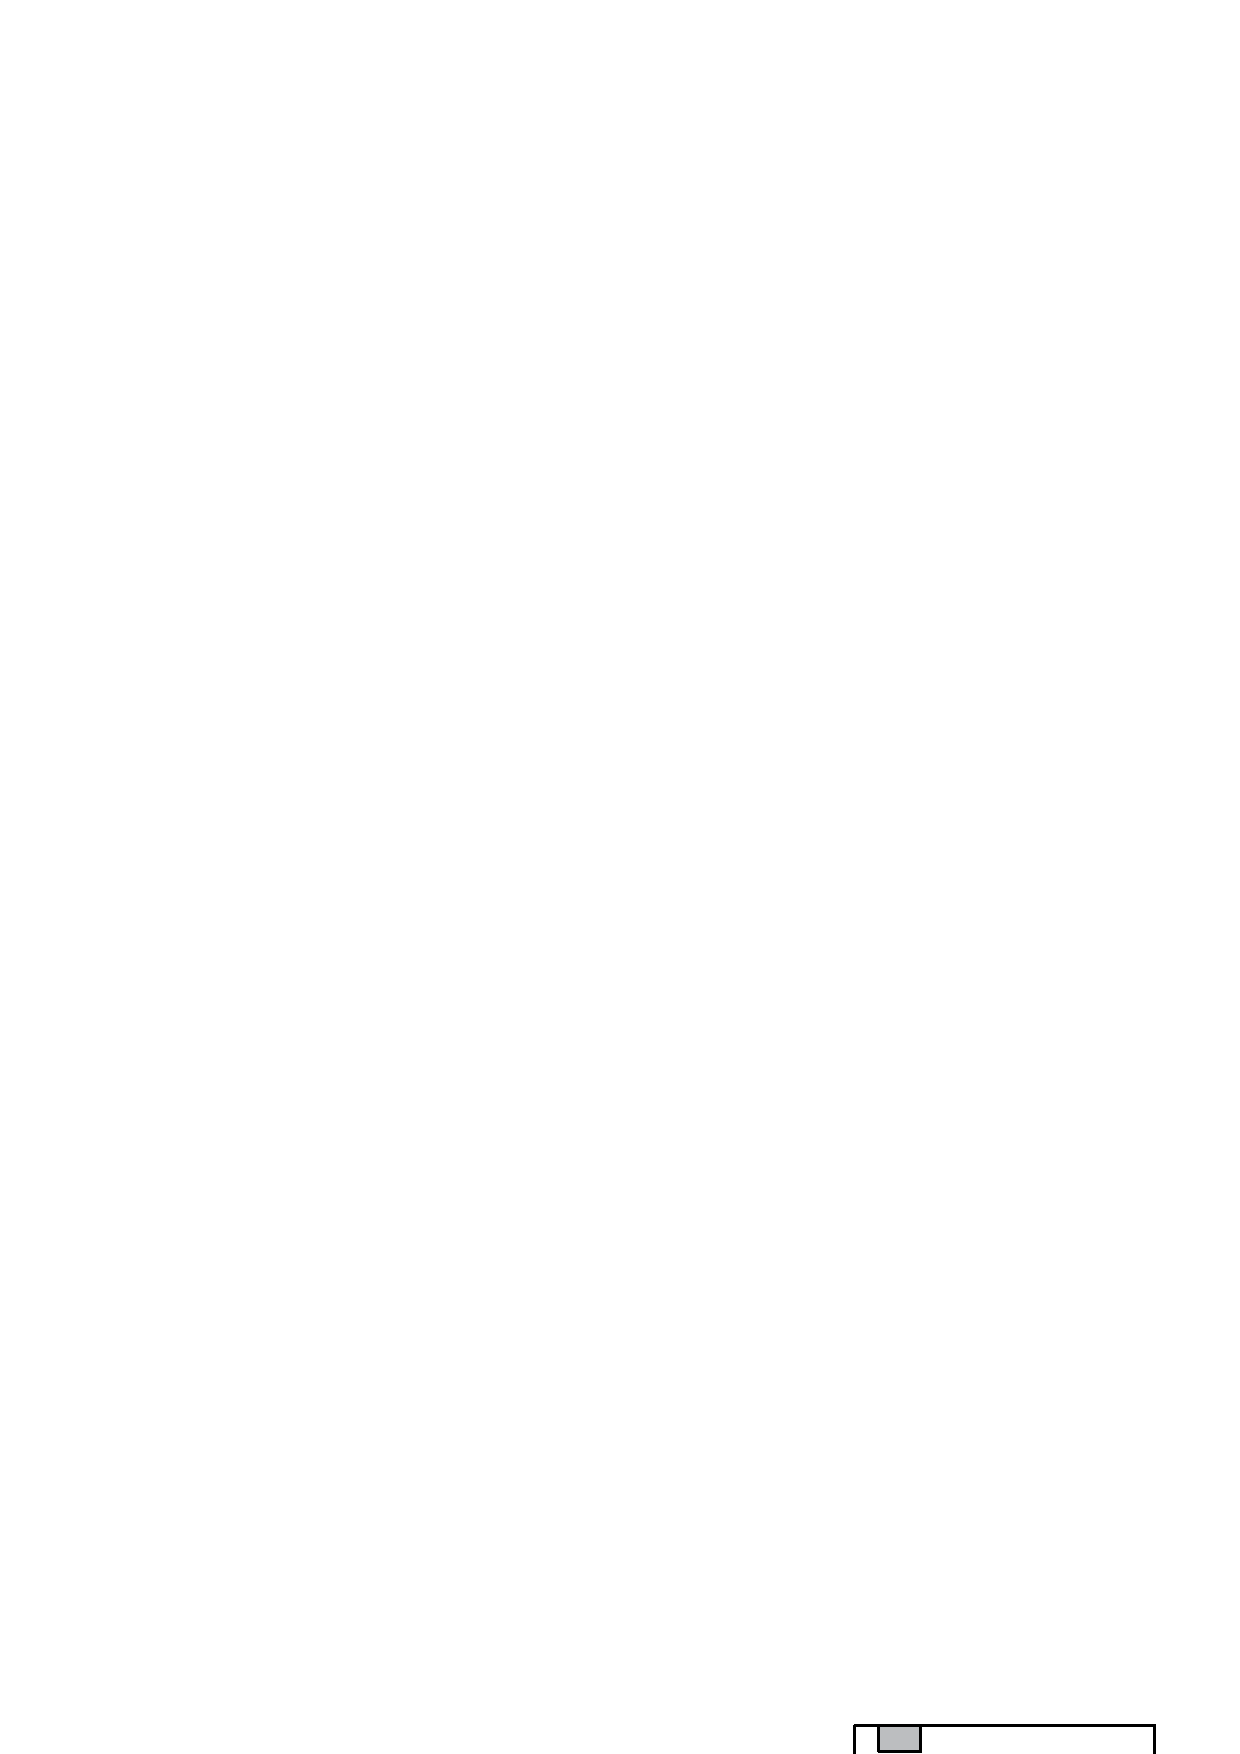
\includegraphics[bb=0 0 768 208,width=\columnwidth]
    {Figures/biopse-modmap.eps.gz}}
}
%end{latexonly}
\begin{htmlonly}
  \newcommand{\basicmodule}{%
  \htmladdimg[align=top,width=766,alt="module"]
  {../Figures/biopse-modmap.gif}}
\end{htmlonly}

The functional unit of a data-flow environment is the {\em\/module}
\index{module}.  Figure~\ref{fig:conc-module} contains a generic \SR{}
module, with a User Interface (UI) button for graphically accessing the
module's user interface, and input and output ports for receiving and sending
data, respectively.  On the right is a simple example of a data-flow
network.  Data passes through the output port of the top module, through
the data pipe, and into the input port of the bottom module.  The User
Interface enables the selection of a desired isochrone surface.

\begin{figure}[htb]
  \begin{makeimage}
  \end{makeimage}
  \basicmodule
  \caption{\label{fig:conc-module} Example of a \SR{} module}
\end{figure}

Modules may contain other elements, but all have at least one input or
one output port. Most modules have input and output ports connected to
other modules.  Data readers are modules with only an output port.
Their ``input'' is read from a file.  The
\module{Viewer} module provides input
ports only; scene data arrives on its input ports and a screen
visualization is its ``output''.  

A \dfn{subnet} is a collection of modules that behave as one.
Sub-Networks can be created, edited, and saved just like networks.
Sub-Networks can be reused in other networks, including other
sub-networks.  Sub-networks simplify the construction of complex
networks.  \sr{} ships with a  set of subnets.  See \secref{Creating a
  Sub-Network}{sec:crsubnet} for details.

It is important to understand the concepts of modules, connections,
networks and data-flow.  See \secref{Working with
  Networks}{ch:workwithnets} for more information on modules, subnets,
ports, connections, and networks.

\section{\sr{}'s Use of Third Party Software}
\label{sec:con-links} 

\SR{} works with software from third party sources in several ways.
The use of third party software is largely invisible to the user of
\SR{} or \BIOPSE{}.

For example, \sr{}'s user interface is written in Tcl language
using the Tk library.  In general, \sr{} modules use Tcl for their
user interface elements and C++ for their computations.  However, a
module may also interact with code written in other languages such as
FORTRAN or Matlab.

One goal of the \BIOPSE{} project is to provide
support for such external code, including FORTRAN, C, Matlab, and
IDL\@.

\subsection{Matlab Interface}
\label{sec:concept-matlab} 
\index{Matlab}

The Matlab interface package allows \sr{} to execute Matlab scripts
and to read and write Matlab matrix data files.

A sockets interface allows \sr{} to exchange a matlab script and matrix
data with a Matlab process.  Matlab executes the script with input
data from \sr{} and returns matrix data to \sr{}.  

The Matlab process can run on the same computer as does \sr{} or it
can run on a separate computer, helping to distribute the load and
resolving potential licensing conflicts with Matlab.

Via the Matlab package, \sr{} can read Matlab matrix files, converting
them to a SCIRun matrix type or a NRRD type.

\subsection{Insight Tool Kit}
\index{Insight Toolkit}

\sr{} provides modules for solving problems in a wide range of areas
such as performance analysis, geometric modeling, numerical analysis,
and scientific visualization.  \sr{}, however, lacks image processing
tools. This deficiency is most prominent in the area of medical
imaging.

The \htmladdnormallinkfoot{Insight Tool Kit}{http://www.itk.org} (ITK)
is open source software that complements \sr{} by providing
image-processing capabilities, ranging from fundamental algorithms to
advanced segmentation and registration tools.  The Insight Tool Kit
provides these capabilities as \dfn{filters}.  \sci{} has developed a
method of encapsulating ITK filters in \sr{} modules.

A simple XML-based language is used to describe the properties of an
ITK filter.  The ITK filter description is independent of the software
system using ITK.  Additional (one or two) \sr{}-specific, XML-based
files drive the module generation process.

If ITK is present (and \sr{} is appropriately configured) \sr{} will
build a default set of ITK filter-based modules.  Users can generate
additional modules by writing XML descriptions. The process of
generating modules based on ITK filters is described in
\chref{Wrapping ITK Filters in \sr Modules}{ch:itk_mods}.

\subsection{PETSc}
\index{PETSc}

\htmladdnormallinkfoot{The Portable, Extensible, Toolkit for
  Scientific Computation
  (PETSc)}{http://www-unix.mcs.anl.gov/petsc/petsc-2/} is a library of
data structures and functions for the parallel solution of partial
differential equations.

When PETSc is installed, and SCIRun is configured to use it, SCIRun's
\module{SolveMatrix} module enables the use of PETSc solvers.

Installation of PETSc is optional.  SolveMatrix provides built-in
solvers if PETSc is not installed.


\subsection{GENESIS (via SQL)}
\index{GENESIS}

\htmladdnormallink{GENESIS}{http://www.bbb.caltech.edu/GENESIS/genesis.html}
(short for GEneral NEural SImulation System) is a general purpose
simulation platform that was developed to support the simulation of neural
systems ranging from complex models of single neurons, to simulations of
large networks made up of more abstract neuronal components. GENESIS has
provided the basis for laboratory courses in neural simulation at
Caltech and the Marine Biological Laboratory in Woods Hole, MA, and 
many other institutions.   

\sci{} has made it possible to use the output of a GENESIS simulation
as the input for a visualization, or a subsequent simulation within
\BIOPSE{}.  The mechanism for this bridge is a database accessible via
SQL queries.  \sci{} created code for GENESIS that writes the output
of the simulation into the database, then the corresponding functions
for \SR{} read this information from the same database.  Contact Chris
Butson
\htmladdnormallink{butson@sci.utah.edu}{mailto:butson@sci.utah.edu}
for details about the implementation of the GENESIS module.


\section{Extensibility}
\label{sec:con-extend} 


\sr{} can be extended by creating new packages, modules, and subnets.
Modules can be coded from scratch, or with the assistance of the \sr's
\dfn{Module Maker} component.

\sci{} encourages users to contribute modules to the \BIOPSE{} web
site \index{BioPSE@\BIOPSE{}!web site}
(\htmladdnormallink{www.sci.utah.edu/ncrr/software/biopse.html}
{http://www.sci.utah.edu/ncrr/software/biopse.html}) where they will be
reviewed, and useful modules will be included in subsequent releases
of \sr{}.

To leverage investment in legacy code, future releases of \sr{} will
include additional tools for wrapping existing code within \SR{}
modules.

\section{Power Apps}
\label{sec:sec:con-apps}
\index{power apps}

SCI is developing problem specific applications called
\dfn{Power Apps}.  Power Apps use \sr{}'s data flow engine for
computation and application specific data flow networks for problem
solving.  However, Power Apps hide the complexity of the data flow
environment behind a simplified application specific graphical user
interface.

The following Power Apps are available:

\begin{description}
  \descitem{BioTensor} \index{BioTensor} An application for computing and visualizing
  diffusion tensor data.  See the \htmladdnormallinkfoot{BioTensor
    tutorial}{\latexhtml{http://software.sci.utah.edu/doc/User/Tutorials/BioTensor/BioTensor.html}{../../Tutorials/BioTensor/BioTensor.html}}
  for more information.
  
  \descitem{BioFEM} \index{BioFEM} A finite element simulation application. It is
  used, for example, to compute electric and potential fields from a
  discretized volume conductor and a current source.
\end{description}

Commands \command{BioTensor} and \command{BioFem} invoke these
applications.  If \sr{} is installed from source code, commands
\command{BioTensor} and \command{BioFem} are located in \sr{}'s build
directory (alongside the \command{scirun} command).  If \sr{} is
installed from RPMs these commands are located in
\directory{/usr/local/SCIRun/bin}.

\section{\sr{} Objects}
\label{sec:sr-objects}

\sr{}'s \datatype{Field}, \datatype{Mesh}, \datatype{Matrix}, and
\datatype{ColorMap} objects are used frequently in networks.  These
objects are described in the following sections.

\subsection{Field}
\index{fields}

A \sr{} \datatype{Field} consists of a geometric \datatype{Mesh} and a
set of data values.  Data values can be located at the nodes, edges,
faces, or cells of a mesh.  A \datatype{Field} can consist of a
\datatype{Mesh} component only (no associated data).

\subsection{Field Data}

The following C++/SCI data types can be associated with a \datatype{Field}:

\begin{itemize}
\item \datatype{double}, \datatype{float}
\item \datatype{int}, \datatype{short}, \datatype{unsigned}, \datatype{unsigned short}
\item \datatype{char}, \datatype{unsigned char}
\item 2nd order \datatype{Tensor}
\item \datatype{Vector} of doubles
\end{itemize}

C++ data types are \datatype{double}, \datatype{float},
\datatype{int}, \datatype{short}, \datatype{unsigned},
\datatype{unsigned short}, \datatype{char}, and \datatype{unsigned
  char}.  \sr{} data types are \datatype{Tensor} and \datatype{Vector}.

\subsection{Meshes}
\index{meshes}

\sr{} meshes are classified as \dfn{unstructured}, \dfn{structured},
or \dfn{regular}.  A mesh consists of nodes and implicit or explicit
node connectivity data.

Node locations and connectivities for unstructured 
meshes\index{meshes!unstructured meshes} are specified
explicitly.  The unstructured mesh types are:
\datatype{PointCloudMesh}, \datatype{CurveMesh},
\datatype{TriSurfMesh}, \datatype{QuadSurfMesh},
\datatype{TetVolMesh}, and \datatype{HexVolMesh}.

Node locations are specified explicitly, and connectivities are known
implicitly for structured meshes\index{meshes!structured meshes}.  The 
structured meshes are
\datatype{StructCurveMesh}, \datatype{StructQuadSurfMesh}, and
\datatype{StructHexVolMesh}.

Node locations and connectivities are known implicitly for regular
meshes\index{meshes!regular meshes}.  The regular mesh types 
are \datatype{ScanlineMesh},
\datatype{ImageMesh}, \datatype{LatVolMesh}.

Below are figures of some mesh types:

%begin{latexonly}
\newcommand{\meshdoc}[4]{%
  \includegraphics[bb=0 0 100 #1]{Figures/#2.eps.gz}
  {#4}
}
%end{latexonly}
\begin{htmlonly}
  \newcommand{\meshdoc}[4]{%
    \htmladdimg[align=left,alt="#3"]
    {../../Tutorials/SCIRun_Intro/images/figures/#2.gif}
    #4 \begin{rawhtml}<br clear="all"/>\end{rawhtml}
  }
\end{htmlonly}

\meshdoc{100}{pointcloud}{Point Cloud Mesh}{A Point Cloud \index{meshes!Point Cloud mesh} mesh is a
  set of unconnected points.}

\meshdoc{60}{ScanlineField}{Scanline Mesh}{A Scanline Mesh \index{meshes!Scanline mesh} is a
  regularly segmented straight line (a regular 1D grid).}

\meshdoc{60}{ContourField}{Contour Field Mesh}{A Curve mesh \index{meshes!Curve mesh} is a 
  segmented curve.}

\meshdoc{100}{ImageField}{Image Mesh}{An Image mesh \index{meshes!Image mesh} is a regular 2D
  grid. Note that an Image mesh is not used for image processing.}

\meshdoc{65}{trisurf}{Tri Surface Mesh}{A Tri Surface mesh \index {meshes!Tri Surface mesh} is a
  surface made of connected triangles.}

\meshdoc{83}{quadsurf}{Quad Surface Mesh}{A Quad Surface \index{meshes!Quad Surface mesh} mesh is a surface made of connected quadrilaterals.}

\meshdoc{87}{latticevol}{Lat Vol Mesh}{A Lattice Volume mesh \index{meshes!Lattice Volume mesh} is a regular 3D grid.}

\meshdoc{60}{tetvol}{Tet Vol Mesh}{A Tet Volume mesh \index{meshes!Tet Volume mesh} is a subdivision of space into tetrahedral elements.}

\meshdoc{84}{hexvol}{Hex Vol Mesh}{A Hex Volume mesh \index{meshes!Hex Volume mesh} is a subdivision
  of space into hexagonal elements.}

%% \meshdoc{?}{prismvol}{Prism Volume Mesh}{A Prism Volume is a
%%   subdivision of space into prism elements.  Prism elements have five
%%   faces, two trangular faces connected by three quadrilateral faces.}

\subsection{Matrices}
\index{matrices}

\sr{} supports three matrix types: 

\begin{description}
\descitem{\datatype{ColumnMatrix}} An \(Mx1\) matrix using \(M\)
storage units.

\descitem{\datatype{DenseMatrix}} An \(MxN\) matrix using \(MxN\)
storage units.

\descitem{\datatype{SparseRowMatrix}} A \(MxN\) matrix where most
elements are zero and no storage is allocated for zero valued
elements.
\end{description}

\subsection{Color Map}
\index{color map}

\sr{} \datatype{ColorMap} type is a mapping of color values to data values.

%%% Local Variables: 
%%% mode: latex
%%% TeX-master: "usersguide"
%%% End: 

% package.tex
%


\section{Packages}
\label{sec:packages}


\subsection{The SCIRun Package}
\label{sec:srpackage}


\subsection{The BioPSE Package}
\label{sec:biopsepackage}


%%% Local Variables: 
%%% mode: latex
%%% TeX-master: "usersguide"
%%% End: 

%
%  For more information, please see: http://software.sci.utah.edu
% 
%  The MIT License
% 
%  Copyright (c) 2004 Scientific Computing and Imaging Institute,
%  University of Utah.
% 
%  License for the specific language governing rights and limitations under
%  Permission is hereby granted, free of charge, to any person obtaining a
%  copy of this software and associated documentation files (the "Software"),
%  to deal in the Software without restriction, including without limitation
%  the rights to use, copy, modify, merge, publish, distribute, sublicense,
%  and/or sell copies of the Software, and to permit persons to whom the
%  Software is furnished to do so, subject to the following conditions:
% 
%  The above copyright notice and this permission notice shall be included
%  in all copies or substantial portions of the Software.
% 
%  THE SOFTWARE IS PROVIDED "AS IS", WITHOUT WARRANTY OF ANY KIND, EXPRESS
%  OR IMPLIED, INCLUDING BUT NOT LIMITED TO THE WARRANTIES OF MERCHANTABILITY,
%  FITNESS FOR A PARTICULAR PURPOSE AND NONINFRINGEMENT. IN NO EVENT SHALL
%  THE AUTHORS OR COPYRIGHT HOLDERS BE LIABLE FOR ANY CLAIM, DAMAGES OR OTHER
%  LIABILITY, WHETHER IN AN ACTION OF CONTRACT, TORT OR OTHERWISE, ARISING
%  FROM, OUT OF OR IN CONNECTION WITH THE SOFTWARE OR THE USE OR OTHER
%  DEALINGS IN THE SOFTWARE.
%


% running.tex
%
% This is the `Running SCIRun' main section.

\chapter{Starting \sr{}}
\label{ch:startingup}


\section{Preparation}
\label{sec:prepare}

Preparations must be made before starting \sr{} and its Power Apps.
Commands below are typed in a terminal emulation application (\eg{}
\command{xterm}).

See \secref{\sr{}'s
Initialization File---\filename{.scirunrc}}{sec:scirunrc} and \secref{Dynamic
Compilation}{sec:dyncomp} for additional information.
  
Mac OSX users must increase the open files limit.
Users of csh-type shells on Mac OSX must type:

\begin{alltt}
  limit descriptors unlimited
\end{alltt}

and users of sh-type shells must type:

\begin{alltt}
  ulimit -n unlimited
\end{alltt}

It is convenient to place the above  in a shell initialization
file (\filename{.cshrc} or \filename{.bashrc}).

%begin{latexonly}
\newcommand{\srwindow}{%
  \centerline{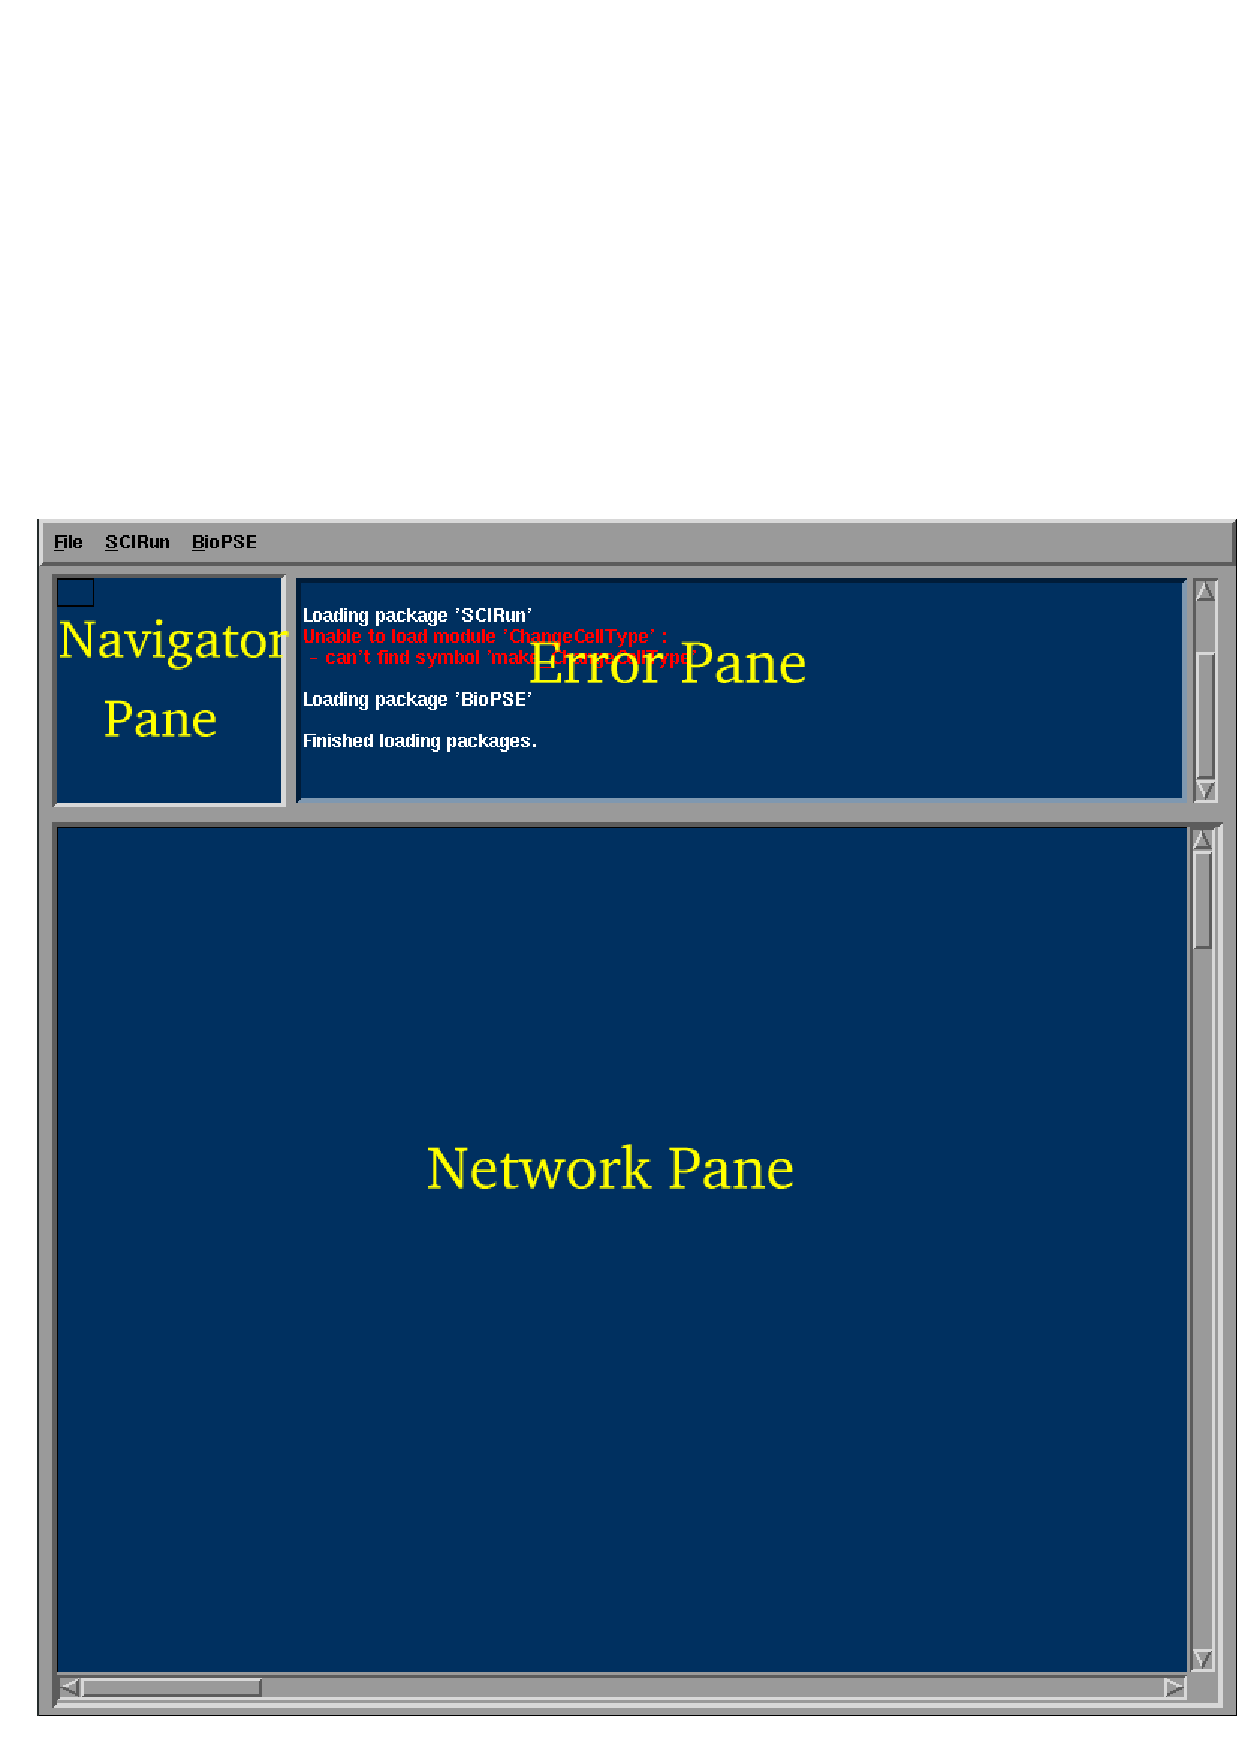
\includegraphics[bb=0 0 391 402,width=4in]{Figures/srwindow-1.eps.gz}}
}
%end{latexonly}
\begin{htmlonly}
  \newcommand{\srwindow}{%
    \htmladdimg[alt="SCIRun Window"]{../Figures/srwindow-1.gif}
  }
\end{htmlonly}

Change your current working directory to \sr{}'s
build directory (for an installation from source code) or to
\filename{/usr/local/SCIRun/bin} (for an installation from an RPM):

\begin{alltt}
  cd SCIRun/sgi32
\end{alltt}

or

\begin{alltt}
  cd /usr/local/SCIRun/bin
\end{alltt}

and type:

\begin{alltt}
  ./scirun [ [-e] \replaceable{network_file} ]
\end{alltt}

\note{Do not start \sr{} in the background, \ie do not type:
  \keyboard{scirun~\&}.}

The \command{scirun} command may take the name of a
\dfn{\sr{} network file} (network files have a \filename{.net} extension)
for \sr{} to load.  The \option{-e} tells \sr{} to execute the network
after it is loaded.  Network files are discussed in a later section.

If the name of a network file is not provided, \sr{} starts with an empty
  window as shown in Figure~\ref{fig:srwindow}.  \secref{Anatomy
  of the Main Window}{sec:windowanatomy} discusses the main features
of Main Window window.

\begin{figure}[htb]
  \begin{makeimage}
  \end{makeimage}
  \srwindow
  \caption{\label{fig:srwindow} \sr{} Main Window}
\end{figure}

\sr{} may encounter errors during start up.  Errors, warnings, and
other messages are displayed in \sr{}'s Message frame (see
Figure~\ref{fig:srwindow}).  Errors should be
\htmladdnormallink{reported}{\bugsurl} to the \sr{} development team
(See \secref{Reporting Bugs}{sec:bugs} for information on reporting
bugs).

\section{Anatomy of the Main Window}
\label{sec:windowanatomy}

The \sr{} main window consists of the Menu Bar, the Global View frame,
the Message frame, and the Net Edit frame (see
Figure~\ref{fig:srwindow}):

\begin{description}
  \descitem{Menu Bar} The menu bar is used to load networks, save
  networks, quit \sr{}, create network modules, and perform other
  tasks.  The menu bar consists of the following menu items:

  \begin{description}
    \menudesc{File} The \menu{File} menu contains the following items:

    \begin{description}
      \menuitemdesc{Load} Loads a network from a file (See
      \hyperref{this section}{Section~}{}{sec:opennet}).
      
      \menuitemdesc{Insert} Adds a network to the NetEdit frame
      without overlap (See \hyperref{this
        section}{Section~}{}{sec:insertnetwork}).
      
      \menuitemdesc{Save} Saves a network to a file (See \hyperref{this
        section}{Section~}{}{sec:savenet}).

      \menuitemdesc{Save As...} Saves a network to a new file (See
      \hyperref{this section}{Section~}{}{sec:savenet}).
      
      \menuitemdesc{Clear Network} Removes all modules and connections from
      the NetEdit frame (See \hyperref{this
        section}{Section~}{}{sec:clearnetwork}).

      \menuitemdesc{Select All} Selects all modules.

      \menuitemdesc{Execute All} Executes all modules.
      
      \menuitemdesc{New} Contains items of interest to
      developers only (e.g. creating new modules).
      
      \menuitemdesc{Add Info} Adds network specific
      notes to the current network.  Notes should be used to document
      the purpose of the network (See \hyperref{this
        section}{Section~}{}{sec:docnetwork}).
    
      \menuitemdesc{Quit} Quits \sr{}.  Pressing key combination
      \keyboard{Control + Q} also quits.
    \end{description}
  \end{description}
  
  \begin{description}
    \menudesc{SCIRun} The \menu{SCIRun} menu is used to create modules
    (from the \sr{} package) for use in the Net Edit frame.

    This menu is composed of sub-menus. Each sub-menu corresponds to
     a \dfn{category}
    \index{category} within the \sr{} package.  A category is a group of
    related modules.  Each menu item in a category sub-menu creates a
    specific module and places it in the NetEdit frame.  
    
    The NetEdit frame pop-up menu  also
    provides access to the \menu{\sr{}} and \menu{\biopse{}} (and
    possibly other) package menus. Activate the NetEdit frame pop-up
    menu by clicking Btn3 (right mouse button). \secref{The
      \biopse{}Package}{sec:biopsepackage} has an overview of the
    \sr{} package.
  \end{description}

  \begin{description}
    \menudesc{BioPSE} The \menu{BioPSE} menu creates modules (from the
    \biopse package) for use in the NetEdit frame.  It consists of
    category sub-menus and module menu items \secref{The SCIRun
      Package}{sec:srpackage} has an overview of the \biopse{}package.
  \end{description}

  \begin{description}
    \descitem{\ptext{Other Package Menus}} There may be other
    package menus if other packages have been installed.  They also
    have category sub-menus and module menu items.
  \end{description}
  
  \descitem{Global View Frame} \index{global view frame}
  The Global View Frame is located in the
  upper left corner of the main window (see
  Figure~\ref{fig:srwindow}). It is used to navigate complex networks
  \secref{Navigating a Network}{sec:navnetwork} describes the use of the Global View Frame.
  
  \descitem{Message Frame} \index{message frame}
  Messages during program startup are displayed
  in the Message frame.  The Message frame is located in the upper right
  corner of the main window (see Figure~\ref{fig:srwindow}).  Errors on
  startup may mean \sr{} has been installed incorrectly or has
  been installed from a buggy distribution.  Please report these
  errors (\hyperref{report}{see Section~}{)}{sec:bugs}).
  
  \descitem{NetEdit Frame} \index{netedit frame}
  The NetEdit Frame occupies the bottom of
  the main window(see Figure~\ref{fig:srwindow}).  It is used to build
  and execute networks (\secref{Working with  Networks}{ch:workwithnets}
  discusses the use of the NetEdit frame).

\end{description}

The Global View, Message, and Net Edit frames can be resized by moving
their borders vertically/horizontally.  The horizontal border separating
the Net Edit frame from the Global View and Message frames can be moved
up or down.  The vertical border separating the Global View and Error
frames can be moved left or right.  To resize a frame, position the
mouse pointer over a border, press (and hold) mouse button 1, and drag
the mouse.  A frame is removed entirely from view by dragging a border
to the window's edge.


\section{The Terminal Window}
\label{sec:termwinapp}

After starting, \sr{} runs a shell-like application in the
terminal window called the \dfn{\sr{} shell}.  The \sr{} shell displays the
prompt \screen{scirun\ra}.  This program is  a modified \dfna{Tool
  Command Language}{TCL} shell program. It is possible to type
\acronym{TCL}'ish \sr{} commands at the prompt.  \hyperref{A later
  section}{Section~}{}{sec:termapp} describes use of the SCIRun shell.


\section{\sr{}'s Initialization File---\filename{.scirunrc}}
\label{sec:scirunrc}
\index{environment variables}
\index{scirunrc}

\sr{} processes \filename{.scirunrc} file on startup.  File
\filename{.scirunrc} contains assignments to environment variables
that affect \sr{}'s behavior.  Lines beginning with '\#' are ignored.

When started by a user the first time, \sr{} creates a default version of
\filename{.scirunrc} in the user's home directory.  Users may modify
their default \filename{.scirunrc} file.

Users may also set \sr{} related environment variables in their
shell.  Values of variables set in the shell override values set in
\filename{.scirunrc}.

See the content of \filename{.scirunrc} for a complete list of \sr{}
related environment variables.  The following
is a partial list of variables understood by \sr{}:

\newcommand{\envitem}[1]{\item[\envvar{#1}]\latex{\mbox{}\\}}

\begin{description}
  \envitem{SCIRUN\_ON\_THE\_FLY\_LIBS\_DIR}
  \envvar{SCIRUN\_ON\_THE\_FLY\_LIBS\_DIR} specifies the location of
  dynamically generated code (see \secref{Dynamic
    Compilation}{sec:dyncomp} for details on the meaning and use of
  this variable).  Users shouldn't need to change the default value
  (\filename{\ltilde/on-the-fly-libs}) of this variable.
  
  \envitem{SCIRUN\_CONFIRM\_OVERWRITE}
  \envvar{SCIRUN\_CONFIRM\_OVERWRITE} determines the default behavior of
  file saving operations.  If set to 1, the user is
  asked to confirm a save operation if an existing file would be
  overwritten.  If set to 0 then the user is not asked for
  confirmation.  \envvar{SCIRUN\_CONFIRM\_OVERWRITE}'s default value is 1.
  
  \descitem{\envvar{SCIRUN\_DATA}, \envvar{SCIRUN\_DATASET}} These two
  variables specify the complete path to a \sr{} \dfn{data set}. A
  data set is a collection of \sr{} type data fields, matrices, \etc{}
  that are stored in a directory and used in \sr{} networks.

  \envvar{SCIRUN\_DATA} specifies a directory that contains a
  collection of data set directories.  \envvar{SCIRUN\_DATA} is used in
  conjunction with \envvar{SCIRUN\_DATASET} to specify the full path of
  a data set.  \envvar{SCIRUN\_DATASET} specifies a specific data set
  directory. 

  When working with the sample \sr{} data sets, for example,
  \envvar{SCIRUN\_DATA} is set to
  \filename{/usr/local/SCIRunData} (assuming this is where \sr{}'s
  sample data were installed).  \envvar{SCIRUN\_DATASET} can then be
  set to \filename{utahtorso} to specify the Utah Torso data set.
  
  \envitem{SCIRUN\_NET\_SUBSTITUTE\_DATADIR} When saving a network
  containing a reader or writer module, \sr{} normally records (in the
  network file) the absolute
  pathname of a reader/writer module's chosen file.  If
  \envvar{SCIRUN\_NET\_SUBSTITUTE\_DATADIR} is set to 1 and if a
  reader/writer module is set to read/write from/to a file in
  \icode{\$SCIRUN\_DATA/\$SCIRUN\_DATASET} then \sr{} will record a
  filename whose path will be determined by future values of
  \envvar{SCIRUN\_DATA} and \envvar{SCIRUN\_DATASET}.  The default
  value of \envvar{SCIRUN\_NET\_SUBSTITUTE\_DATADIR} is 0.

  \envitem{SCIRUN\_TMP\_DIR}
  \envvar{SCIRUN\_TMP\_DIR} specifies the directory where \sr{} will
  create temporary files.  It's default value is \filename{/tmp}.

  \envitem{SCIRUN\_LOAD\_PACKAGE}
  \envvar{SCIRUN\_LOAD\_PACKAGE} is a comma separated list of packages
  \sr{} is to load upon startup.  Normally \sr{} loads all installed
  packages.  To load, for example, only the \BIOPSE{} and Teem
  packages: \envvar{SCIRUN\_LOAD\_PACKAGE=BioPSE,Teem}.

  \envitem{SCIRUN\_NOSPLASH}
  If \envvar{SCIRUN\_NOSPLASH} is set to 1, then \sr{} will not display
  its splash screen at startup.  The default value is 0.

  \envitem{SCIRUN\_HIDE\_PROGRESS}
  If \envvar{SCIRUN\_HIDE\_PROGRESS} is set to 1, \sr{} will not display
  progress bars during startup.  The default value is 0.
  
  \envitem{SCIRUN\_STRAIGHT\_CONNECTIONS}
  If \envvar{SCIRUN\_STRAIGHT\_CONNECTIONS} is set to 1, \sr{} will draw
  straight connections between modules in the Network Editor.  The
  default value of \envvar{SCIRUN\_STRAIGHT\_CONNECTIONS} is 0.

  \envitem{SCIRUN\_FAST\_QUIT} If defined, disables the confirmation
  dialog that is normally displayed when exiting \sr.
  
  \envitem{SCIRUN\_MPEG\_LICENSE\_ACCEPT} MPEG software is freely
  distributed with \sr{} and may be used for any non-commercial
  purpose.  However, patents are held by several companies on various
  aspects of the MPEG video standard. Companies or individuals who
  want to develop commercial products that include this code must
  acquire licenses from these companies. For information on licensing,
  see Appendix F in the standard. For more information, please see the
  README file in the mpeg\_encode distribution. If you are allowed to
  use the MPEG functionality based on the above license, you may
  enable MPEG movie recording in SCIRun (accessible via the SCIRun
  Viewer's "File->Record Movie" menu) by setting the value of
  SCIRUN\_MPEG\_LICENSE\_ACCEPT to "true".
\end{description}

\section{Remote Display}
\label{sec:remote-display}
\index{remote display}

Normally, \sr{}'s main window is displayed on a console that is part
of the computer on which \sr{} runs.  It is possible, however, to
display \sr{} on a \dfn{remote} console.  In the discussion that
follows, the term \dfn{local} refers to the machine running \sr{} and
the term \dfn{remote} refers to the machine displaying \sr{}.

To display \sr{} remotely, the value of the \envvar{DISPLAY}
environment variable must be set correctly on the local machine.
Also, the local machine must be allowed to send display commands to
the remote machine.
  
Normally, the remote machine makes a connection to the local machine
via the \command{ssh} command.  In this case, \command{ssh} sets the value of
\envvar{DISPLAY} in such a way that the local machine has permission to
send display commands to the remote machine.  However, \command{ssh}
connections result in poor display performance because of encryption
activity on the connection.

To increase performance, the value of \envvar{DISPLAY} is set as
follows after establishing the \command{ssh} connection:

for a sh-style shell

\begin{verbatim}
  export DISPLAY=remote-machine-name:0.0
\end{verbatim}
  
for a csh-style shell

\begin{verbatim}
  setenv DISPLAY remote-machine-name:0.0
\end{verbatim}

Note that this technique defeats the encryption protection on the
connection.

After overriding the value of \envvar{DISPLAY} set by \command{ssh},
the local machine will lack permission to send display commands to the
remote machine.  Use the \command{xhost} command on the remote machine
to give permission to the local machine:

\begin{verbatim}
  xhost +local-machine-name
\end{verbatim}
  

\section{Dynamic Compilation}
\label{sec:dyncomp}
\index{dynamic compilation}

Before executing \sr{},  be aware of the
\dfn{Dynamic Compilation} feature.

Dynamic compilation is a technique used by \sr{} to discover and
generate code for data types and algorithms used by modules in
networks.  This is done at runtime and once for each new
data type and algorithm encountered.  This technique provides a number
of benefits not discussed here (see the publication 
\htmladdnormallinkfoot{\etitle{Dynamic
    Compilation of C++ Template Code}}{http://www.sci.utah.edu/publications/mcole01/dyn.pdf}
for details).

By default, code generated by dynamic compilation is stored in
directory \directory{on-the-fly-libs} in the user's home directory.
The location of dynamically generated code can be changed by setting
the value of the environment variable
\envvar{SCIRUN\_ON\_THE\_FLY\_LIBS\_DIR} to the desired directory.

For example:

for Bourne-like shells (sh, ksh, bash, etc,)

\begin{verbatim}
SCIRUN_ON_THE_FLY_LIBS_DIR=~/SCIRun/on-the-fly-libs
export SCIRUN_ON_THE_FLY_LIBS_DIR
\end{verbatim}

for csh-like shells

\begin{verbatim}
setenv SCIRUN_ON_THE_FLY_LIBS_DIR ~/SCIRun/on-the-fly-libs
\end{verbatim}

SCIRUN\_ON\_THE\_FLY\_LIBS\_DIR can be set in the user's
\filename{.scirunrc} file.

\begin{verbatim}
SCIRUN_ON_THE_FLY_LIBS_DIR=/home/me/on-the-fly-libs
\end{verbatim}

Setting a unique value of SCIRUN\_ON\_THE\_FLY\_LIBS\_DIR for each
\sr{} user has the following benefits:

\begin{itemize}
\item Allows multiple users \index{multiple users} to run the same 
  instance of \sr{} without
  dynamic compilation conflicts.  For example, by specifying an
  \filename{on-the-fly-libs} directory in their home directory, a user
  can run \sr{} installed in \directory{/usr/local} that another user
  is already running.

\item Allows a \directory{/usr/local} installation of \sr{}
  to be secure because it does not require
  \directory{/usr/local/.../on-the-fly-libs} to be writable by
  all (a potential security risk).

\item Allows greater debugging and multiple build support by
  allowing the user to change dynamically compiled code locations
  between instances of \sr{}.

\end{itemize}

Dynamic compilation causes a delay the first time a module is
executed.  The module changes color while it is being
compiled.

\section{Exiting \sr{}}
\label{sec:stopping}

Exit \sr{} by selecting the \menuitem{Quit} item from the \menu{File}
menu or by pressing \keyboard{control-q}.

Do not press \keyboard{control-c} to exit \sr{}.  Doing this will drop
\sr{} into a debugger.

% network.tex
%
% The Working with networks section.

%begin{latexonly}
  \newcommand{\modgraphic}%
  {\centerline{\epsfig{file=figures/modgraphic.eps,width=\columnwidth}}}
%end{latexonly}
\begin{htmlonly}
  \newcommand{\srwindow}{%
  \htmladdimg[align=top,width=6,alt="SCIRun Window"]
  {../figures/modgraphic.gif}}
\end{htmlonly}

\section{Working with Networks}
\label{sec:workwithnets}

This section describes how to create, save, open, execute, and edit
networks.

Starting \sr\ (with no arguments) will create the \sr\ main window with a
blank network pane window.  The goal then is to build a network by
creating and connecting modules.


\subsection{Creating a Module}
\label{sec:creatingmodules}

Create a module by selecting its name from one of the package (\eg \sr)
menu's category submenu.  The package menus may be accessed from the main
window's menu bar and from the network pane's popup menu.

Activate the network pane's popup menu by clicking  mouse
button 3 while the mouse pointer is in the network pane.  The popup menu
contains a list of category submenus from the \sr package and any
additional packages.  And of course each category submenu provides access
to the modules within the category.

After creating a module its graphic ``front end'' will be created and
placed in the network pane.

\subsubsection{Anatomy of a Module}
\label{sec:modanatomy}

All modules are represented similarly by a graphic within the network pane.
See Figure~\ref{fig:modgraphic}. For all modules this graphical ``front
end'' consists of the following components:

\begin{description}
\item[Name] The module's name.
\item[Input ports] Zero or more input ports.  Each port corresponds to a
  data type and each data type has a unique color.
  Table~\ref{tab:portcolors} maps port colors to data types.  Input ports
  connect to other modules' output ports.  Connections can only be made
  between ports of the same type.
\item[Output ports] Zero or more output ports.  Output ports connect to
  other modules' input ports.  Every module has, of course, at least 1 input
  or 1 output port.
\item[UI button] Pressing the \button{UI} button displays the module's
  control dialog. Some modules have no such dialog. Some have very
  simple dialogs.  Some have very complex dialogs which allow elaborate
  control over the module.  
\item[Progress bar] Shows the module's progress.
\item[Timer] Displays the amount of CPU time the module has consumed.
  Located to the left of the progress bar.
\item[Popup Menu] Pressing mouse button 3 while the mouse
  pointer is over a module gives access to the module's popup menu.  The
  popup menu gives access to the following items:
  \begin{description}
  \item[::Package_Category_Name_Instance] This item is a label (not a
    selectable item).  It provides the module's name and the category and
    package to which to module belongs.  The Instance part is a unique
    number which distinguishes multiple instances of the same module.
  \item[\menuitem{Execute}] Executes the network.
  \item[\menuitem{Notes}] This item displays the module's note pad.  Use the note pad
    to document the purpose of the module in the current network.
  \item[\menuitem{Destroy}] Destroys the module.
  \item[\menuitem{Show Log}] Displays the module's message log.  Most modules will
    write messages to the log during the course of their execution.
  \item[\menuitem{Show Status}] This item is a toggle button which turns off/on the
    display of the progress indicator.  Turning off the progress indicator
    can help speed up the execution of complex networks.
  \end{description}
\end{description}

\begin{table}[htbp]
  \begin{center}
    \begin{tabular}{|l|l|}
      \textbf{Data Type} & \textbf{Port Color} \\
      \hline
      Field & Yellow \\
      Field Set & Green \\
      Matricies & Blue \\
      Geometric Objects & Pink \\
      Color Maps & Purple \\
      Camera Path & Brown \\
      \hline
    \end{tabular}
    \caption{Data Types and their Port Colors}
    \label{tab:portcolors}
  \end{center}
\end{table}


\begin{figure}[htb]
  \begin{makeimage}
  \end{makeimage}
  \modgraphic
%  \centerline{\epsfig{file=figures/modgraphic.eps,width=6in}}
  \caption{\label{fig:module} \sr\ module}
\end{figure}


\subsection{Making a Connection}
\label{sec:connectmods}

Button 2 is used to connect the input port of one module to
the output port of another module (or vice-versa).  

Position the mouse pointer over a module's input (output) port.  Then press
button 2 and drag the the mouse pointer towards another module's output (input)
port.   

When button 2 is first pressed the program shows all valid connections as
black lines.  It also draws one red colored connection which is the
connection that will be made if you stop the drag by releasing the mouse
button.

Make the final connection by releasing button 2 when the pointer is over
the desired destination port or when the red colored connection is the
desired one.

The connection will be drawn using an appropriate data type color.

\subsection{Deleting a Connection}
\label{sec:deleteconnections}

A connection may be deleted by pressing button 3 while the pointer is
over a connection.

\subsection{Moving a  Module}
\label{sec:movemod}

Modules may be moved around in the network pane.  To move a module simply
press button 1 while the pointer is over a module and drag the module to
its new location.

\subsection{Changing a Module's Properties}
\label{sec:setmodprops}

To change a module's properties click its \button{UI} button.  This will
display the module's control dialog.  Use this dialog to change the
module's properties.  Each module's reference documentation explains the
use of its control dialog.


\subsection{Deleting (Destroying) a Module}
\label{sec:deletemod}

Delete a module by selecting the \menuitem{Destroy} menu item from the
module's popup menu.

\subsection{Executing a Network}
\label{sec:executenet}


\subsection{Documenting a Module}
\label{sec:docmodule}

It is often useful to document the purpose of a module within a network.
Each module maintains a note pad for this purpose.  You may edit the
module's note pad by selecting \menuitem{Notes} item from the module's
popup menu.  This will display the module's note pad editor.  This simple
editor allows you to write notes or otherwise document the use of the
module within the context of its network.

\subsection{Viewing a Module's Log}
\label{sec:viewmodslog}

Each module supports a message log.  The module may write error messages or
other types of messages to its log.  To view this log select the
\menuitem{Show Log} item from the module's popup menu.

\subsection{Documenting a Network}
\label{sec:docnetwork}

It is useful to document the purpose of a network.  You may use a network's
note pad for this purpose.  To edit the network's note pad select the
\menuitem{Add Info} item from the main window's \menu{File} menu.  This
will display the network's note pad editor.  This simple editor allows you
to write notes or otherwise document the purpose and use of the network.


\subsection{Saving a Network}
\label{sec:savenet}

To save a network select the \menuitem{Save} item from the main window's
\menu{File} menu.


\subsection{Opening a Network}
\label{sec:opennet}

To open a network select the \menuitem{Open} item from the main window's
\menu{File} menu.


\subsection{Navigating a Network}
\label{sec:navnetwork}

A complex network may not be entirely visible in the network pane.  You may
use the network pane's scroll bars to bring other parts of a network into
view.  Or you may use the navigation tool to view complex networks.

The navigation pane shows the entire ``network world.''  The small
rectangular region (outlined in black) within the navigation pane is the
network navigation tool and it is a window on the network world.  The
position of the navigation tool determines which part of the network is
visible in the network pane.  To view other parts of the network, press
button 1 while the pointer is anywhere in the navigation pane (this will
move the tool to the location of the pointer) and then drag the tool to the
new location.



%%% Local Variables: 
%%% mode: latex
%%% TeX-master: "usersguide"
%%% End: 

% -*-latex-*-
%
%  The contents of this file are subject to the University of Utah Public
%  License (the "License"); you may not use this file except in compliance
%  with the License.
%
%  Software distributed under the License is distributed on an "AS IS"
%  basis, WITHOUT WARRANTY OF ANY KIND, either express or implied. See the
%  License for the specific language governing rights and limitations under
%  the License.
%
%  The Original Source Code is SCIRun, released March 12, 2001.
%
%  The Original Source Code was developed by the University of Utah.
%  Portions created by UNIVERSITY are Copyright (C) 2001, 1994
%  University of Utah. All Rights Reserved.
%

%%%%%%%%%%  Figures used in this file %%%%%%%%%%%%%%%%%%%%%%%%%%%%%%%%
%% The basic viewer window
%begin{latexonly}
  \newcommand{\viewerwindow}%
  {\centerline{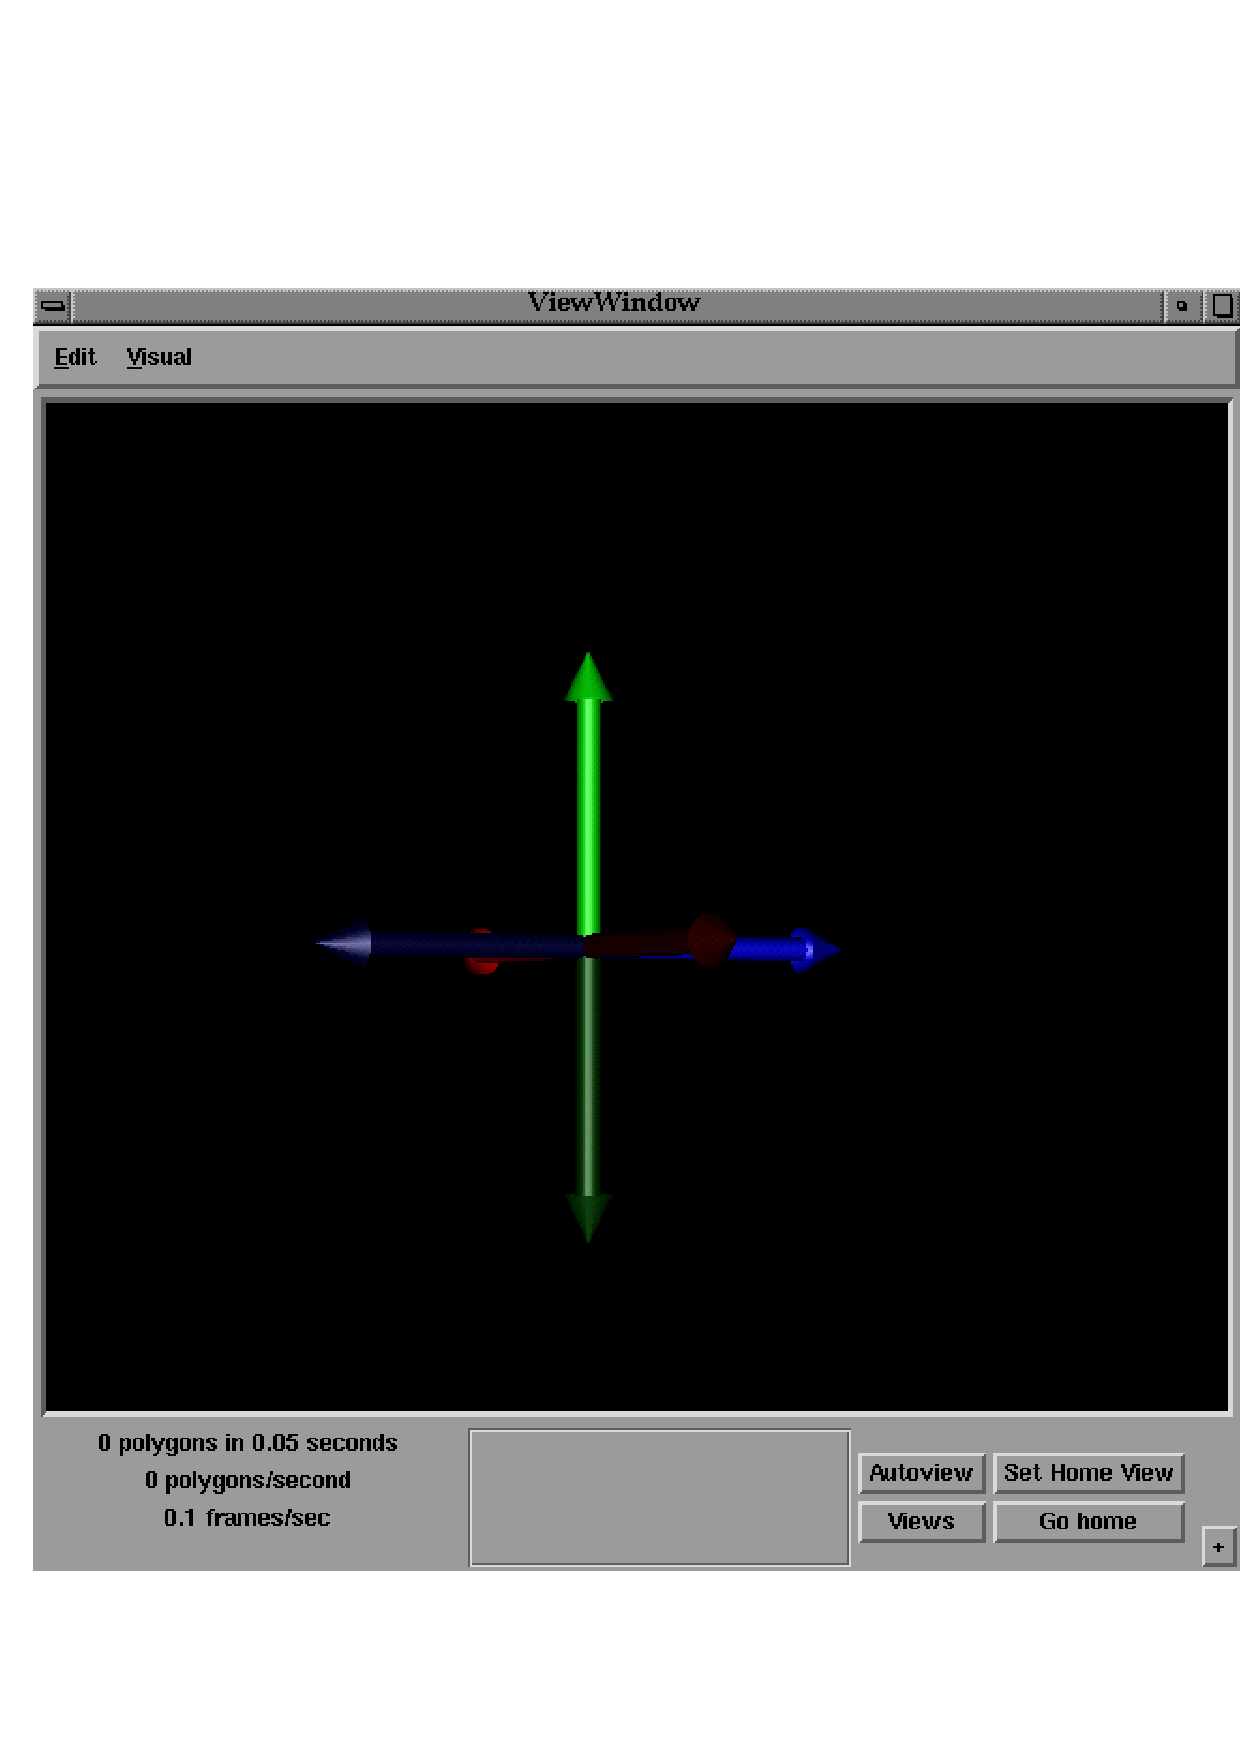
\epsfig{file=Figures/viewwindow.eps.gz,height=4in,
  bbllx=0, bblly=0, bburx=660, bbury=660}}}
%end{latexonly}
\begin{htmlonly}
  \newcommand{\viewerwindow}{%
  \htmladdimg[align=top,width=645,alt="module"]
  {../Figures/viewwindow.gif}}
\end{htmlonly}

%% View of the extended viewer window
%begin{latexonly}
  \newcommand{\extendedwindow}%
  {\centerline{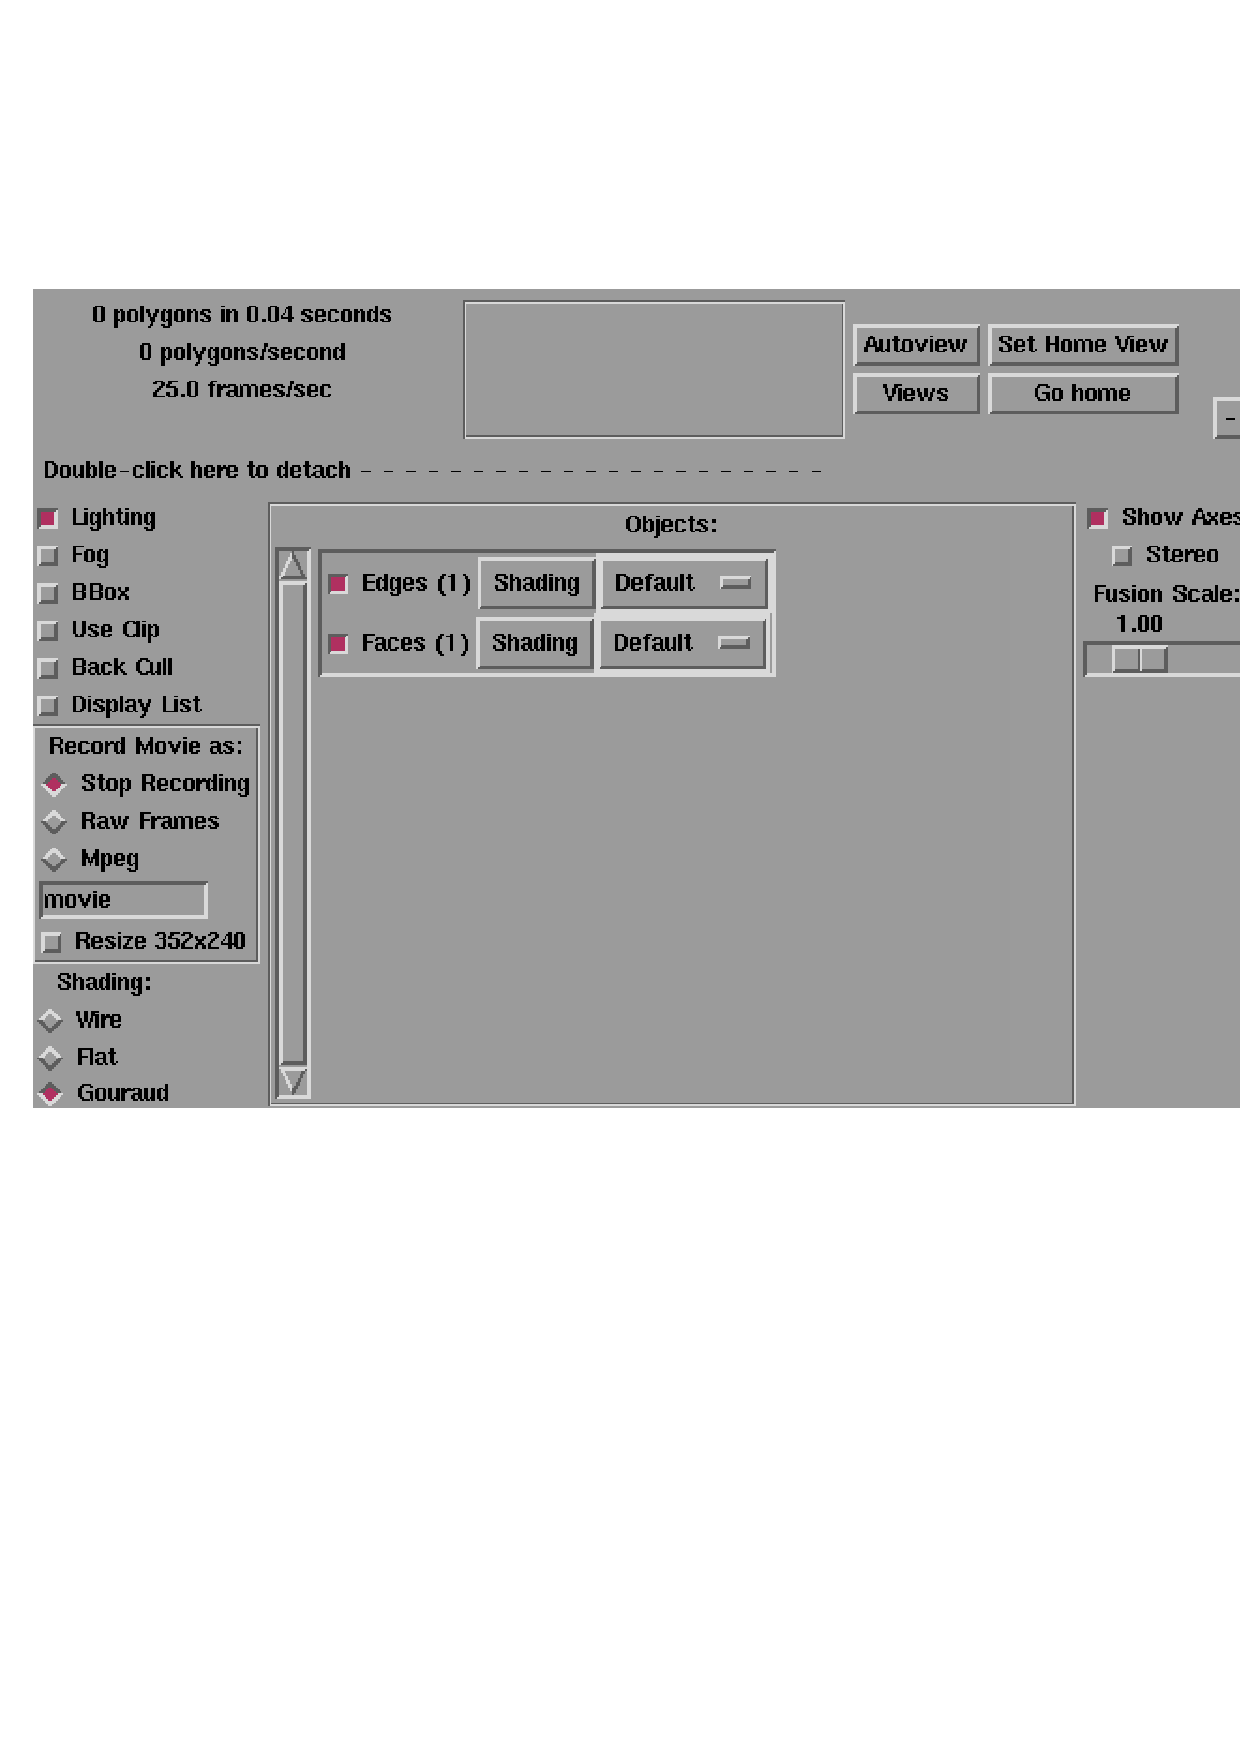
\epsfig{file=Figures/viewwindow-ext.eps.gz,height=4in,
  bbllx=16, bblly=310, bburx=600, bbury=703}}}
%end{latexonly}
\begin{htmlonly}
  \newcommand{\extendedwindow}{%
  \htmladdimg[align=top,width=649,alt="extended view window"]
  {../Figures/viewwindow-ext.jpg}}
\end{htmlonly}

%% Gauge widget image
%begin{latexonly}
  \newcommand{\gaugewidget}%
  {\centerline{\epsfig{file=Figures/widget-gauge.eps.gz,height=2in,
  bbllx=0, bblly=0, bburx=457, bbury=340}}}
%end{latexonly}
\begin{htmlonly}
  \newcommand{\gaugewidget}{%
  \htmladdimg[align=top,width=458,alt="gaugewidget"]
  {../Figures/widget-gauge.gif}}
\end{htmlonly}

%% Frame widget image
%begin{latexonly}
  \newcommand{\framewidget}%
  {\centerline{\epsfig{file=Figures/widget-frame.eps.gz,height=2in,
  bbllx=0, bblly=0, bburx=328, bbury=268}}}
%end{latexonly}
\begin{htmlonly}
  \newcommand{\framewidget}{%
  \htmladdimg[align=top,width=329,alt="framewidget"]
  {../Figures/widget-frame.gif}}
\end{htmlonly}

%% Box widget image
%begin{latexonly}
  \newcommand{\boxwidget}%
  {\centerline{\epsfig{file=Figures/widget-box.eps.gz,height=2in,
  bbllx=0, bblly=0, bburx=458, bbury=342}}}
%end{latexonly}
\begin{htmlonly}
  \newcommand{\boxwidget}{%
  \htmladdimg[align=top,width=459,alt="boxwidget"]
  {../Figures/widget-box.gif}}
\end{htmlonly}

%% Ring widget image
%begin{latexonly}
  \newcommand{\ringwidget}%
  {\centerline{\epsfig{file=Figures/widget-ring.eps.gz,height=2in,
  bbllx=0, bblly=0, bburx=507, bbury=467}}}
%end{latexonly}
\begin{htmlonly}
  \newcommand{\ringwidget}{%
  \htmladdimg[align=top,width=508,alt="ringwidget"]
  {../Figures/widget-ring.gif}}
\end{htmlonly}

%%%%%%%%%%%%%%%%%%%%%%%%%%%%%%%%%%%%%%%%%%%%%%%%%%%%%%%%%%%%%%%%%%%%%%
\newcommand{\graphics}{\emph{Graphics}}

\section{Visualization with the \viewer{}}
\label{sec:viewer}
\index{Viewer@\viewer{}}

This section describes the most frequently used \sr{} module,
the \viewer{}, which has the task of displaying interactive graphical
output to the computer screen.  You will use the \viewer{} any time you
wish to see a geometry, or spatial data.  More important for
computational steering (described in \secref{Computational
Steering}{sec:con-steering}) is that the \viewer{} provides access to
many simulation parameters and controls and thus indirectly initiates new
iterations of the simulation steps.

We begin with an overview of the \viewer{} window and its controls, then
describe in detail all the options and variations.

\subsection{Anatomy of the \viewer{} window}
\label{sec:viewer-anatomy} 
\index{Viewer@\viewer{}!anatomy}

The \viewer{} window contains two main areas, the upper portion,
called the \graphics{} window, which displays the graphics, and the
lower portion, where most of the control buttons are.
Figure~\ref{fig:viewwindow} contains an example of a \viewer{} window.
In the \graphics{} window, viewing is controlled mostly by means of the
mouse, mouse buttons, and various modifier keys (shift/control/alt).
In the lower window are a lot of buttons and sliders, the function of
which will become clear as you read this section of the manual.

\begin{figure}[htb]
  \begin{makeimage}
  \end{makeimage}
  \viewerwindow
%    \framebox{\parbox[3in]{\columnwidth}{The\dotfill Figure\\
%    \vspace{2in}\\
%    With some \dotfill dummy text}}
  \caption{\label{fig:viewwindow} The default \viewer{} window in \SR{}}
\end{figure}


First, try out the controls for the \graphics{} window by moving the mouse
to the center of the viewer window and clicking and holding the left button
and then dragging the mouse.  The objects should translate along with the
mouse.  Do the same operation with the middle mouse button and the objects
will rotate around a point in the center of the display.  The right mouse
button controls the scale of the display, zooming in when the mouse moves
downward or to the right.  See \secref{Mouse Control in the
Viewer}{sec:view-mouse} for details on using the mouse.

The controls visible along the bottom of the \viewer{} window set some basic
configurations as follows:
%
\begin{description}
\item [\button{Autoview}]\mbox{}
  
  Restores the display to a default condition. Very useful when some
  combination of settings results in the objects disappearing from the
  view window.

\item [\button{Set Home View}]\mbox{}
  
  Captures the setting of the current view so you can return to it
  later by clicking the Go home'' button.

\item [\button{Go home}]\mbox{}

  Restore the current home view.

\item [\button{Views}]\mbox{}
  
  Lists a number of standard viewing angles and orientations.  The
  view directions align with the Cartesian axes of the objects and the
  ``Up vector'' choice sets the orientation of the objects when viewed
  along the selected axis.

\end{description}

In the left corner of the control panel of the \viewer{} window are
performance indicators that document the current rendering speed for the
display.  The better the graphics performance of the workstation you
have, the higher the display rate.

You may reveal more controls by clicking the
\latexhtml{\fbox{+}}{\button{[+]}} button in the lower right corner of
the \viewer{} window.  The extended controls are described in
\secref{Extended control window} {sec:view-control}.


\subsubsection{Menus}
\index{Viewer@\viewer{}!menus}

At the top of the \viewer{} window are three pull-down menus.

\begin{description}
  \item [\menu{File}] \mbox{}

    Current contains only the \menuitem{Save image file...} item which
    allows you to save the contents of the \viewer{} window as an
    image to a file.

  \item [\menu{Edit}]\mbox{} 
    
    Provides access to controls for the background color for the
    window, as well as the clipping planes (requires the ``Use Clip''
    control to be selected in the extended controls described in
    \secref{Extended control window}{sec:view-control}).

  \item [\menu{Visual}]\mbox{}
    
    Allows you to select between different graphics hardware settings
    that are available on your workstation.  The list is ordered
    heuristically from most to least useful.

\end{description}

\subsection{Mouse Control in the \viewer{} Window}
\label{sec:view-mouse} 
\index{Viewer@\viewer{}!mouse controls}

The mouse controls within \SR{} are extensive and flexible.  The
resulting action depends on the choice of mouse button, any
simultaneously pressed control keys, and the way the mouse moves.  The
description in Tables~\ref{tab:view-mouse} and~\ref{tab:view-unicam}
below may seem overly complicated at first, but with a little playing,
it becomes intuitive (another way of saying you will learn it if you
use it enough).

\begin{table}[htb]
\begin{center}
  \begin{tabular}{|l|l|p{5in}|} \hline
    \multicolumn{3}{|c|}{\large Mouse Controls}\\ \hline \hline 
    \multicolumn{1}{|c|}{Control Key} & 
    \multicolumn{1}{|c|}{Button} & 
    \multicolumn{1}{|c|}{Action}\\ \hline
None & Left & Translate scene \\
     & Middle & \begin{raggedleft} Rotate scene about its center on an arc
    ball that surrounds it; rotation direction is a function of the
    initial mouse location so try different sites and note the
    response. \end{raggedleft}\\  
     & Right & Zoom or scale scene (downwards and to the right increases
     size, upwards or to the left decreases size) \\ \hline
Shift & Left & Select and move a widget in the display \\
      & Middle & Toggle through the modes for a widget \\
      & Right & Pop up a widget information window \\ \hline
Control & Left & Translate in the Z-direction, \ie{} zoom in and out of the
    screen (down moves closer, up further away).  Moving left and
    right increases the ``throttle'' of the Z-direction motion.  If
    the cursor is over a point on an object when clicked, this point
    becomes the center of the screen for translation.\\ 
      & Middle & Rotate the camera view about the eye point (using arcball
    motion). \\ 
      & Right & Unicam movement (see Table~\ref{tab:view-unicam})\\ \hline
\end{tabular}
\caption{\label{tab:view-mouse} Mouse controls for the \viewer{}}
\end{center}
\end{table}

\bigskip

\begin{table}
\begin{center}
\begin{tabular}{|l|l|p{3in}|} \hline
    \multicolumn{3}{|c|}{\large Unicam movement (Control key and right mouse
    button} \\ \hline \hline
    \multicolumn{1}{|c|}{Initial mouse location} & 
    \multicolumn{1}{|c|}{Action} & \\ 
    \hline
    Near edge of display & Rotate objects on the arc ball & \\
    Near the objects & Following behavior: & \\
    \hline
    & \multicolumn{1}{|c|}{Initial mouse movement} & 
    \multicolumn{1}{|c|}{Action}\\ \hline
    & Horizontal & Pan objects \\ 
    & Vertical & Zoom and pan: down = zoom in, up = zoom
    out, left and right= pan left and right) \\
    & None & Set rotation point for subsequent arc ball rotation.\\
    \hline
\end{tabular}
\caption{\label{tab:view-unicam} Autocam mouse controls in the \viewer{}}
\end{center}
\end{table}



\subsection{Extended Control Window}
\label{sec:view-control} 
\index{Viewer@\viewer{}!extended controls}

Click on the \button{[+]} button in the lower right corner of the
default \viewer{} window, and the window expands to reveal an extended
panel of control buttons, as shown in Figure~\ref{fig:extviewwindow}.
Click on the \button{[-]} sign that now replaces the \button{[+]} and
this extended panel disappears again.  Here we describe the control
options available in the extended control window.

\begin{figure}[htb]
  \begin{makeimage}
  \end{makeimage}
  \extendedwindow
%    \framebox{\parbox[3in]{\columnwidth}{The\dotfill Figure\\
%    \vspace{2in}\\
%    With some \dotfill dummy text}}
  \caption{\label{fig:extviewwindow} The lower portion of extended
    \viewer{} window in \SR{}} 
\end{figure}


\subsubsection{Object selector}

The lower portion of the extended \viewer{} window is divided into three
columns. The middle column contains a list of all the objects in the
display.  If the list becomes long enough, a scroll bar on the left
hand side controls which are visible.  For each entry in the list, we have
the following controls, reading from left to right:

\begin{itemize}
  \item At the left end of each of the
        objects in the list is a selection indicator that displays red
        when that object is 
        selected.  The \viewer{} window only displays those objects that
        are selected.
  \item Next comes the name of the object.
  \item The \button{Shading} control box that comes next determines the
        shading options that will be used for rendering the object.
        Options include: Lighting, BBox, Fog, Use Clip, Back Cull, and
        Display List (for descriptions, see
        \secref{Rendering controls}{sec:view-rendering}).
  \item At the right end of each entry is the lighting control, initially
        marked \menu{Default}.  In the Default setting, the common
        rendering controls described in \secref{Rendering
        controls}{sec:view-rendering} below apply.  Clicking this box
        reveals a set of options that will apply only to this object that
        include Wire, Flat and Gouraud.
\end{itemize}


\subsubsection{Rendering Controls}
\label{sec:view-rendering} 
\index{Viewer@\viewer{}!rendering}

The left column of the extended \viewer{} window contains controls that
apply to all of the selected objects with ``Default'' lighting selected.
Those without the Default setting will use their own, object specific
settings, as described in the previous section.  The lighting and shading
options available are:
%
\begin{description}
  \item [Lighting] Toggles whether or not the \viewer{} applies lighting
        to the display.  Objects without lighting have a constant
        color.
  \item [Fog] Draws objects with variable intensity based on their
        distance from the user, also known as ``depth cueing''.  Close
        objects appear brighter while more remote objects fade gradually
        into the background as a function of distance from the front.
  \item [BBox] Toggles whether the \viewer{} draws the selected objects
        in full detail or as a simple bounding box.
  \item [Use Clip] Applies up to six clipping planes to the display.
        To control the clipping plane locations, use the
        ``Edit -\ra{} Clipping Planes'' menu at the top of the
        \viewer{} window.
  \item [Back Cull] Displays only the forward facing facets of any surface
        objects in the display.
  \item [Display List] Cache the list of objects to be displayed; this
        option accelerates rendering when the content of the display does
        not change. 
  \item [Shading] Selects the type of shading for objects from the
        following options:
        \begin{description}
          \item [Wire] Show only the wire mesh of objects.
          \item [Flat] Draw each facet with a constant color.
          \item [Gouraud] Linearly interpolate the color across facets. 
        \end{description}
\end{description}

The right hand column of the extended \viewer{} window contains controls
for displaying the axes and creating stereoscopic rendering.  

\paragraph{Stereo viewing: } requires hardware LCD glasses synchronized
with the display so that visibility for each eye coincides with the
display of the appropriate view.  The ``Fusion Scale'' control provides a
means of setting the eye separation and thus setting the view that is most
suited to facial anatomy and distance from the screen.

\subsubsection{Making movies}
\label{sec:view-movies} 
\index{movies}

The \viewer{} window in \SR{} has simple controls for capturing sequences
of images into animations or movies.  Here we describe how this works.

In the left column of the extended \viewer{} window are controls for
selecting movie type and then initiating and stopping the acquisition of
individual frames in the movie.

\SR{} sends a frame to the movie after each ``redraw'' operation, \ie{}
each time anything moves in the display or any visualization parameter
changes.  If the MPEG package is available (See the
\htmladdnormallink{Installation Manual}{\installguideurl} for
details) then an option will be available for saving the animations as MPEG
movies.

There is also a button that forces the size of the graphical window to be
352x240 pixels in size, which is a standard format well suited to MPEG.

\subsection{Control widgets}
\label{sec:view-widgets} 

While the \hyperref{mouse controls}{mouse controls in
Section}{}{sec:view-mouse} describe many ways to interact with the contents
of the \viewer{}, SR{} also supports some powerful display widgets.
Examples of widgets capabilities include managing cutting surfaces colored
according to the local data values, displaying streamlines in vector
fields, or selecting sub-volumes within the display area for further
manipulation. 
 
We have tried to make interacting with these widgets as consistent as
possible so that, for example, controlling parameters is usually by clicking
and dragging on either a cylindrical ``collar'' or a sphere element of the
widget.  The original design of these modules was by James Purcifal
%%\cite{??}. 
Note that a single widget may have more than one purpose
depending on the context in which it exists.

In this section, we describe the widgets available within \SR{} and \BIOPSE{}.
The same widget may, for example, select a clipping or a display plane
through a three-dimensional object but may also set the seed points for a
streamline module.  

\subsubsection{Gauge Widget}
\label{sec:view-gaugewidget} 

\begin{figure}[htb]
  \begin{makeimage}
  \end{makeimage}
  \gaugewidget
%    \framebox{\parbox[3in]{\columnwidth}{The\dotfill Figure\\
%    \vspace{2in}\\
%    With some \dotfill dummy text}}
  \caption{\label{fig:gaugewidget} The gauge widget for setting location and
    density of seed points}
\end{figure}

\paragraph{Appearance: } The Gauge Widget consists of two spheres (A)
connected by a cylinder (B) with a small slider collar (C) on the cylinder.
There are also small resize cylinders extending from the spheres (D).

\paragraph{Purpose:} The primary use of the Gauge Widget is to set the
location and density of streamlines emerging from the long cylinder.  It
may also be used as a more general purpose three-dimensional slider or as a
source for a stream surface. 

\paragraph{Controls: } Clicking and dragging either sphere causes the
entire widget to move in space, rotating about the other sphere and
following along behind the selected sphere.  Dragging either of the resize
cylinders cases the size of the widget to change and dragging any point on
the main cylinder moves the whole widget without any change in orientation.
Dragging the slider collar changes the associated value, typically the
density of seed points for a streamline source.

\subsubsection{Frame Widget}
\label{sec:view-framewidget} 

\begin{figure}[htb]
  \begin{makeimage}
  \end{makeimage}
  \framewidget
%    \framebox{\parbox[3in]{\columnwidth}{The\dotfill Figure\\
%    \vspace{2in}\\
%    With some \dotfill dummy text}}
  \caption{\label{fig:framewidget} The frame widget for selecting
    cutting/projection planes}
\end{figure}


\paragraph{Appearance: } The Frame Widget consists of four cylinders
connected in a rectangle.  In the middle of each of the cylinders there is
a sphere (B), from which a resize cylinder extends (C).

\paragraph{Purpose:} The primary uses of the Frame Widget is for image
plane definition, for defining stream volumes, and as a "tie dye" as with
the Ring Widget described in \secref{Ring Widget}{sec:view-ringwidget}.

\paragraph{Controls: } Clicking and ragging a sphere on the widget will
cause the widget to rotate about it center; dragging on a resize cylinder
will move the associated edge and this extend or contract the rectangle.
Dragging any of the cylinder will drag the entire widget through space.


\subsubsection{Box Widget}
\label{sec:view-boxwidget} 

\begin{figure}[htb]
  \begin{makeimage}
  \end{makeimage}
  \boxwidget
%    \framebox{\parbox[3in]{\columnwidth}{The\dotfill Figure\\
%    \vspace{2in}\\
%    With some \dotfill dummy text}}
  \caption{\label{fig:boxwidget} The boxwidget for selecting sub-volumes}
\end{figure}

\paragraph{Appearance: } The Box Widget consists of twelve cylinders (A)
connected in a hexahedral box (three-dimensional rectangle) with cylinders
indicating on the edges of the box (B).  In the middle of each face of the
box is a sphere with a cylinder protruding from it (C) that provide resize
control.

\paragraph{Purpose:} The primary use of the Box Widget is to select a
subvolume of the workspace for further manipulation (\eg{} volume
rendering, isosurfaces, streamlines, mesh adaption) where the faces of the
widget act as orthogonal clipping planes.

\paragraph{Controls: } Clicking and dragging on one of the spheres rotates
the widget about its center without changing the position of the center.
Clicking on and dragging any resize handle
% What do these look like??
causes the associated face to extend without changing its orientation.
Dragging a cylinder causes the entire widget to move without changing its
orientation.

\subsubsection{Ring Widget}
\label{sec:view-ringwidget} 

\begin{figure}[htb]
  \begin{makeimage}
  \end{makeimage}
  \ringwidget
%    \framebox{\parbox[3in]{\columnwidth}{The\dotfill Figure\\
%    \vspace{2in}\\
%    With some \dotfill dummy text}}
  \caption{\label{fig:ringwidget} The ring widget for selecting
    cutting/projection planes}
\end{figure}


\paragraph{Appearance: } The Ring Widget consists of a ring (A) with four
embedded spheres (B), each with a resize cylindrical attached (D).  Between
two of the spheres is a sliding collar (C).  One of the resize cylinders
has a special material property (typically a different color from the other
cylinders) to indicate that it is the ``halfway point'' for the slider (E).

\paragraph{Purpose:} The primary use of the Ring Widget is to set the
density of streamlines emerging from the ring---the ring serves as a set of
seed points from which will emerge streamlines.  The Ring Widget can also
serve as a three-dimensional angle gauge, as a source for multiple
streamlines throughout its surface, as a source for a stream surface from
the outer ring, and as a source for a stream volume.  Another use is as a
color sheet, or ``tie dye'', in which the surface is colored as a function of
the scalar value of the field at each point.

\paragraph{Controls: } Clicking and dragging the slider collar along the
ring changes the density of the seed points or some other related
parameter.  Dragging the spheres controls the orientation of the Ring
Widget, while moving the resize cylinders changes the radius of the Ring
Widget about its center.  Dragging any other point on the ring moves the
ring in space without changing its radius or orientation.


%%% Local Variables: 
%%% mode: latex
%%% TeX-master: t
%%% End: 

%
%  For more information, please see: http://software.sci.utah.edu
% 
%  The MIT License
% 
%  Copyright (c) 2004 Scientific Computing and Imaging Institute,
%  University of Utah.
% 
%  License for the specific language governing rights and limitations under
%  Permission is hereby granted, free of charge, to any person obtaining a
%  copy of this software and associated documentation files (the "Software"),
%  to deal in the Software without restriction, including without limitation
%  the rights to use, copy, modify, merge, publish, distribute, sublicense,
%  and/or sell copies of the Software, and to permit persons to whom the
%  Software is furnished to do so, subject to the following conditions:
% 
%  The above copyright notice and this permission notice shall be included
%  in all copies or substantial portions of the Software.
% 
%  THE SOFTWARE IS PROVIDED "AS IS", WITHOUT WARRANTY OF ANY KIND, EXPRESS
%  OR IMPLIED, INCLUDING BUT NOT LIMITED TO THE WARRANTIES OF MERCHANTABILITY,
%  FITNESS FOR A PARTICULAR PURPOSE AND NONINFRINGEMENT. IN NO EVENT SHALL
%  THE AUTHORS OR COPYRIGHT HOLDERS BE LIABLE FOR ANY CLAIM, DAMAGES OR OTHER
%  LIABILITY, WHETHER IN AN ACTION OF CONTRACT, TORT OR OTHERWISE, ARISING
%  FROM, OUT OF OR IN CONNECTION WITH THE SOFTWARE OR THE USE OR OTHER
%  DEALINGS IN THE SOFTWARE.
%


\chapter{Importing and Exporting \sr{} Data}
\label{ch:import_export} 
\index{importing}
\index{exporting}

This chapter describes the format of text-based data files and the use
of \sr{}'s reader and writer modules to import/export \sr{} data
objects from/to text files. 

\sr{}'s reader and writer modules support two classes of data formats:
\sr{}'s persistent format and text-based formats.  \sr{}'s persistent
format supports binary and ascii representations.  \sr{}'s persistent
ascii format is not commonly used and is not discussed further.  This
chapter discusses the text-based formats only.

In general, it is best to save data in \sr{}'s persistent binary
format because data saved in this format loads faster, supports better
numerical precision, and is usually smaller than its text-based
counterparts.  \sr{}'s binary data files are portable between machine
architectures.  Text-based data are used primarily to import data
generated by other software into \sr{} and to export \sr{} generated
data to other software.

\sr{}'s fields, matrices, and color maps can be stored in either type
of file although fields with regular meshes can only be stored in
\sr{}'s binary format.  Fields with regular meshes can be
imported/exported using the \package{Teem} package.  See
\htmladdnormallinkfoot{\package{Teem} file format
  documentation}{http://www.cs.utah.edu/~gk/teem/nrrd/format.html} and
\htmladdnormallinkfoot{\package{Teem} module
  descriptions}{\latexhtml{\scisoftware{}/doc}{../../..}/Developer/Modules/Teem.html}
for information.

\section{Text-based File Formats}

\sr{}'s reader and writer modules read and write text files containing the
following data:

\begin{itemize}
\item Node coordinates
\item Node connectivities
\item Structured mesh parameters
\item Column matrices
\item Dense matrices
\item Sparse row matrices
\item Color map parameters
\end{itemize}

\sr{} unstructured field types are stored in two or three text files.
Curve, hex volume, quad surface, tet volume, and tri surface fields
each require three files: a \secrefalt{node
  coordinate}{sec:node_loc_fmt}, a
\secrefalt{connectivity}{sec:node_conn_fmt}, and a \secrefalt{column
  matrix}{sec:colmat} file.  Point cloud fields require no
connectivity file.  

Note that field readers read node coordinate and connectivity files
only.  Therefore, to construct a complete field from text-based files
a \module{FieldReader} module is used to read node coordinate and
connectivity data and a \module{MatrixReader} module is used to read
field data from a matrix file.  Outputs from modules
\module{FieldReader} and \module{FieldReader} are sent to module
\module{ManageFieldData}, which combines their outputs to create
complete field object.  See \secref{Using Readers}{sec:using_readers}
for more information.

When writing a field, use module \module{ManageFieldData} to split a
field into a geometry stream and a data stream.  Send the geometry
stream to module \module{FieldWriter}, which writes node coordinate
and connectivity files, and send the data stream to module
\module{MatrixWriter}, which writes field data to a matrix file.  See
\secref{Using Writers}{sec:using_writers} for more information.

The structured (curve, quad surface, and hex volume) field types each
require only a \secrefalt{node coordinate}{sec:struct_meshes} file.

\sr{} column matrix, dense matrix, and sparse row matrix data are
stored in \secrefalt{column matrix}{sec:colmat}, \secrefalt{dense
  matrix}{sec:dense_matrix} and \secrefalt{sparse
  matrix}{sec:sparse_row_matrix} files respectively.

A Colormap is stored in a \secrefalt{colormap}{sec:colormap_fmt} file.

\subsection{Node Coordinate File}
\label{sec:node_loc_fmt}

Node coordinate files have the extension \filename{.pts}.  A node
coordinate file contains the coordinates of every node in a mesh.

Field reader and writer modules import/export pts files.

The format is as follows:

\begin{verbatim}
N
x0 y0 z0
x1 y1 z1
    .
    .
    .
xN yN zN
\end{verbatim}

\verb|N| is the number of nodes in the file.  Each remaining line
defines the coordinates of one mesh node.

\subsection{Connectivity Files}
\label{sec:node_conn_fmt}

\sr{} supports five unstructured mesh types.  Each mesh type is
described by a corresponding type of node connectivity file.  Curve
meshes are made up of edge elements contained in \dfn{edge} files.
Surface meshes composed of triangular elements are stored in \dfn{fac}
files.  Surface meshes composed of quadrilateral elements are stored
in \dfn{quad} files.  Volume meshes composed of tetrahedral elements
are stored in \dfn{tet} files.  Volume meshes composed of hexahedral
elements are stored in \dfn{hex} file.

Edge files have the file extension \filename{.edge}.  Fac files have
the extension \filename{.fac}.  Likewise for quad, tet, and hex files.

Field reader and writer modules import/export edge, fac, quad, tet,
and hex connectivity files.

Connectivity files are formatted as follows:

\begin{verbatim}
N
Node indicies of element 0
Node indicies of element 1
            .
            .
            .
Node indicies of element N
\end{verbatim}

\verb|N| specifies the number of elements in a file.

Each  remaining line specifies node indices of one element.
Node indices are assumed to be zero-based.

Edge files have two node indices per line, fac files have three, quad
and tet files have four, and hex files have eight node indices per
line.  For example, a fac file looks like the following:

\begin{verbatim}
N
i0 j0 k0
i1 j1 k0
    .
    .
    .
iN jN kN
\end{verbatim}


%% Needs work!
\subsection{Structured Meshes}
\label{sec:struct_meshes}

Structured meshes are stored in node coordinate (pts) files.  Only
node coordinates are needed.  Connectivities are implicit because node
coordinates are stored in \dfn{scan-line} order.

For example, in a structured hexahedral mesh, the list of nodes comprising
element \(e_{i,j,k}\) is \(\{n_{i,j,k}, n_{i,j,k+1}, n_{i,j+1,k+1}, n_{i,j+1,k}, n_{i+1,j,k}, n_{i+1,j,k+1}, n_{i+1,j+1,k+1}, n_{i+1,j+1,k}\}\)

% Verify the following paragraph.  See converter source code.
The formats of node coordinate files for structured meshes differ
slightly from node coordinate files described in \secref{Node
  Coordinate File Format}{sec:node_loc_fmt}.  Node coordinate files
for structured meshes specify the number of indices in each dimension
of the mesh.

A structured curve field node coordinate file looks like this:

\begin{verbatim}
NI
x0 y0 z0
x1 y1 z1
    .
    .
    .
xN yN zN
\end{verbatim}

The node coordinate file for a structured quadrilateral surface field
looks like this:

\begin{verbatim}
NI NJ
x0 y0 z0
x1 y1 z1
    .
    .
    .
xN yN zN
\end{verbatim}

The node coordinate file for a structured hexahedral volume field
looks like this:

\begin{verbatim}
NI NJ NK
x0 y0 z0
x1 y1 z1
    .
    .
    .
xN yN zN
\end{verbatim}


\subsection{Column Matrix}
\label{sec:colmat}

The column matrix file format is:

\begin{verbatim}
N
v0 
v1
.
.
.
vN
\end{verbatim}

\verb|N| specifies the number of matrix rows.  \verb|N| is followed by
a list of data values.

\subsection{Dense Matrix}
\label{sec:dense_matrix}

The dense matrix file format is:

\begin{verbatim}
N M
v(0,0) v(0,1)...v(0,M)
v(1,0) v(1,1)...v(1,M)
        .
        .
        .
v(N,0) v(N,1)...v(N,M)
\end{verbatim}

\verb|N|, \verb|M| are the number of matrix rows and columns
respectively.  Following \verb|N| and \verb|M| is a list of data
values given in row major order.


\subsection{Sparse Row Matrix}
\label{sec:sparse_row_matrix}

The sparse row matrix file format is:

\begin{verbatim}
NR NC NE
r0 c0 v0
r1 c1 v1
   .
   .
   .
rNE cNE vNE
\end{verbatim}

\verb|NR|, \verb|NC|, and \verb|NE| specify the number of rows, number
of columns, and number of matrix entries respectively.  

Remaining lines are matrix entries.  Each entry consists of a row
index, a column index, and a data value.  Entries must have ascending
row indices. Column indices must be in ascending order for rows with
multiple entries.

\subsection{Color Map}
\label{sec:colormap_fmt}

The color map file format is:

\begin{verbatim}
N
r1 g1 b1 a1 v1
r2 g2 b2 a2 v2
      .
      .
      .
rN gN bN aN vN
\end{verbatim}


\verb|N| specifies the number of color map entries in the file.

Each line following \verb|N| is a color map entry consisting of an RGB
color entry, an alpha value, and a data value.  All RGB, alpha, and
data values are in the range 0.0 to 1.0 inclusive.


\section{Using Readers}
\label{sec:using_readers}

%begin{latexonly}
\newcommand{\MatrixReaderGUI}{%
  \centerline{\includegraphics[bb=0 0 485 252]{Figures/MatrixReaderGUI.eps.gz}}
}
%end{latexonly}
\begin{htmlonly}
  \newcommand{\MatrixReaderGUI}{%
    \htmladdimg[alt="MatrixReader Dialog"]{../Figures/MatrixReaderGUI.gif}
  }
\end{htmlonly}

%begin{latexonly}
\newcommand{\ReadFieldNet}{%
  \centerline{\includegraphics[bb=0 0 358 227,height=2in]{Figures/ReadFieldNet.eps.gz}}
}
%end{latexonly}
\begin{htmlonly}
  \newcommand{\ReadFieldNet}{%
    \htmladdimg[alt="Network that reads a text-based field"]{../Figures/ReadFieldNet.gif}
  }
\end{htmlonly}

Control dialogs for all reader modules are similar.  They contain a
file type popup menu that selects the type (binary or text) of file to
read as input.  The dialog's file browser is used to choose a file.
Figure~\ref{fig:MatrixReaderGUI} shows the control dialog for module
\module{MatrixReader}.  When reading a SCIRun matrix file, item
\guimenuitem{SCIRun Matrix File (*.fld)} is selected from the file
type popup menu.  When reading a text-based matrix file then one of
\guimenuitem{TextDenseMatrix (*.*)} or
\guimenuitem{TextSparseRowMatrix (*.*)} is selected from the file type
popup menu depending on the type of matrix stored in the text file.

\begin{figure}[htb]
  \centering
  \begin{makeimage} \end{makeimage}
  \MatrixReaderGUI
  \caption{\label{fig:MatrixReaderGUI} MatrixReader's dialog}
\end{figure}


When reading unstructured field data from a text file, module
\module{FieldReader} reads data from a node coordinate file and a
separate node connectivity file.  However only one of the files is
chosen with the file browser.  \module{FieldReader} assumes the other
file's name differs only in its extension.

Module \module{FieldReader} can read only field geometry (node
coordinate and node connectivity) data from text files.  Module
\module{MatrixReader} is used to read field data values.  Module
\module{ManageFieldData} is used to merge field geometry data (from
module \module{FieldReader}) with field data values to form a complete
filed.  Figure~\ref{fig:ReadFieldNet} shows the arrangement of these
three modules.

\begin{figure}[htb]
  \centering
  \begin{makeimage} \end{makeimage}
  \ReadFieldNet
  \caption{\label{fig:ReadFieldNet} Network that reads text-based field data}
\end{figure}

\section{Using Writers}
\label{sec:using_writers}

%begin{latexonly}
\newcommand{\FieldWriterGUI}{%
  \centerline{\includegraphics[bb=0 0 434 483,height=4in]{Figures/FieldWriterGUI.eps.gz}}
}
%end{latexonly}
\begin{htmlonly}
  \newcommand{\FieldWriterGUI}{%
    \htmladdimg[alt="FieldWriter dialog"]{../Figures/FieldWriterGUI.gif}
  }
\end{htmlonly}

%begin{latexonly}
\newcommand{\WriteFieldNet}{%
  \centerline{\includegraphics[bb=0 0 387 224,height=2in]{Figures/WriteFieldNet.eps.gz}}
}
%end{latexonly}
\begin{htmlonly}
  \newcommand{\WriteFieldNet}{%
    \htmladdimg[alt="Network that reads a text-based field"]{../Figures/WriteFieldNet.gif}
  }
\end{htmlonly}

Control dialogs for all writer modules are similar.  They contain a file
type popup menu that selects the type (e.g. text or binary) of file
(or possibly files for text output) to write as output.  The dialog's
file browser is used to specify an output file.  Figure~\ref{fig:FieldWriterGUI}
shows the control dialog for module \module{FieldWriter}.  

\begin{figure}[htb]
  \centering
  \begin{makeimage} \end{makeimage}
  \FieldWriterGUI
  \caption{\label{fig:FieldWriterGUI} FieldWriter's dialog}
\end{figure}

When writing unstructured field data to text files, module \module{FieldWriter}
writes data to a node coordinate file and a separate node connectivity
file.  However only one of the files is specified in the dialog.
\module{FieldWriter} assumes the other file's name differs only in its
extension.

When writing to text files, module \module{FieldWriter} can write only
field geometry (node coordinate and node connectivity) data.  Module
\module{FieldWriter} is used to write field data values.  Module
\module{ManageFieldData} is used to split field geometry data from
field data values, sending field geometry data to module
\module{FieldWriter} and field node data to module
\module{FieldWriter}.  Figure~\ref{fig:WriteFieldNet} shows the
arrangement of these three modules.

\begin{figure}[htb]
  \centering
  \begin{makeimage} \end{makeimage}
  \WriteFieldNet
  \caption{\label{fig:WriteFieldNet} Network that writes text-based field data}
\end{figure}




% -*-latex-*-
%
%  The contents of this file are subject to the University of Utah Public
%  License (the "License"); you may not use this file except in compliance
%  with the License.
%
%  Software distributed under the License is distributed on an "AS IS"
%  basis, WITHOUT WARRANTY OF ANY KIND, either express or implied. See the
%  License for the specific language governing rights and limitations under
%  the License.
%
%  The Original Source Code is SCIRun, released March 12, 2001.
%
%  The Original Source Code was developed by the University of Utah.
%  Portions created by UNIVERSITY are Copyright (C) 2001, 1994
%  University of Utah. All Rights Reserved.
%


\chapter{Wrapping  ITK Filters in \sr{} Modules}
\label{ch:itk_mods}

The \htmladdnormallinkfoot{National Library of Medicine Insight
  Segmentation and Registration Toolkit}{http://www.itk.org} (ITK)
is open source software that complements \sr{} by providing
image-processing capabilities, ranging from fundamental algorithms to
advanced segmentation and registration tools.  The Insight Tool Kit
provides these capabilities as \dfn{filters}.  \sci{} has developed a
method of wrapping ITK filters in \sr{} modules.

If ITK is present, and \sr{} is appropriately configured, \sr{} 
builds a default set of ITK filter-based modules.  Users can generate 
additional modules by writing XML descriptions. This chapter describes
the process of wrapping ITK filters in \sr{} modules.

Before reading this chapter, users should be familiar with \sr{}, the
Insight toolkit, and the use of generic programming techniques.  Users
must have access to the \sr{} source code tree and be familiar with
its organization.


\section{Aim}
\label{sec:itk_mods:aim}

ITK filters are C++ objects (also known as \dfn{process objects}) that
receive data on input ports and forward results on output ports.
ITK filter objects provide functions for establishing connections to
ports and setting filter properties.

\sr{} modules are C++ objects that receive data via input ports
and forward results via output ports.  \sr{} modules provide
GUI-based dialogs for modifying  module properties.

The aim of \sr{}/ITK integration is to map ITK filter data types,
ports, properties, and property editing functions to \sr{} module data
types, ports, properties, and property editing GUI dialogs.


\section{Approach}
\label{sec:itk_mods:approach}

ITK filters are mapped onto \sr{} modules via XML description files.
Two  XML files are required for each filter.  A third  file can be created
if a filter requires a custom module GUI.

Software in the \sr{} build
system translates these XML files to \sr{} modules.  The three XML
files are described in \secref{ITK Filter
  Description}{sec:itk_mods:itk_filter_desc}, \secref{\sr{} Filter
  Description}{sec:itk_mods:sr_filter_desc}, and \secref{\sr{} GUI
  Description}{sec:itk_mods:sr_gui_desc}, respectively.


\section{ITK Filter Description}
\label{sec:itk_mods:itk_filter_desc}

The ITK filter description XML file describes a filter's inputs,
outputs, parameters, parameter modifying member functions, templated
data types, and other filter information.  This file contains no \sr{}
specific information.  

ITK filter description files are located in
directory \directory{SCIRun/src/Packages/Insight/ITK}. 
ITK filter description files follow the naming convention:

\begin{alltt}
  itk\_\replaceable{filter_name}.xml
\end{alltt}

for example:

\begin{alltt}
  itk\_BinaryThresholdImageFilter.xml
\end{alltt}


The following XML code illustrates the overall content of an ITK
filter description file:

\begin{alltt}
  <?xml version="1.0" encoding="iso-8859-1"?>
  <!DOCTYPE filter SYSTEM "itk_filter.dtd">
  <filter-itk name="itk::\replaceable{name}">
     <description>
     \velide
     </description>
     <templated>
     \velide
     </templated>
     <datatypes>
     \velide
     </datatypes>
     <inputs>
     \velide
     </inputs>
     <outputs>
     \velide
     </outputs>
     <parameters>
     \velide
     </parameters>
     <includes>
     \velide   
     </includes>
  </filter-itk>
\end{alltt}

Each element is discussed below.

\subsection{Element \xmlstarttag{filter-itk}}
\label{sec:itk_mods:filter-itk_element}

Element \xmlstarttag{filter-itk} is the top-level element.  All other
elements are enclosed in element \xmlstarttag{filter-itk}. The value
of the required ``name'' attribute is the qualified C++ filter name.

For example:

\begin{alltt}
  <filter-itk name="itk::ReflectImageFilter">
    \velide
  </filter>
\end{alltt}

\subsection{Element \xmlstarttag{description}}
\label{sec:itk_mods:descr_element}

Element \xmlstarttag{description} should provide a short (several sentences)
filter description.  

For example:

\begin{alltt}
  <description>
    Implements a Reflection of an image along a selected 
    direction. This class is parameterized over the type 
    of the input image and the type of the output image. 
  </description>
\end{alltt}


\subsection{Element \xmlstarttag{templated}}
\label{sec:itk_mods:templated}

ITK filters are templated (parameterized) C++ classes and generally
support one or two template parameters.  The \xmlstarttag{templated}
element describes a filter's template information.  Specifically, 
\xmlstarttag{templated} contains elements that name a filter's
template parameters and list suitable data types for filter
instantiations.

\begin{alltt}
<templated>
  <template>\replaceable{template\_parameter\_name1}</template>
  <template>\replaceable{template\_parameter\_name2}</template>
  \velide 
  <defaults>
    <default>\replaceable{data\_type\_for\_parameter\_name1}</default>
    <default>\replaceable{data\_type\_for\_parameter\_name2}</default>
    \velide
  </defaults>
  <defaults>
    <default>\replaceable{data\_type\_for\_parameter\_name1}</default>
    <default>\replaceable{data\_type\_for\_parameter\_name2}</default>
    \velide
  </defaults>
  \velide
</templated>
\end{alltt}

Each \xmlstarttag{template} element declares and names a template
parameter.  Template parameter names may be used in subsequent
\xmlstarttag{input} and \xmlstarttag{output} elements---see below.

Each \xmlstarttag{defaults} element corresponds to one filter class
instantiation.  Each \xmlstarttag{default} element names a type that
corresponds (in order) with previous \xmlstarttag{template} elements.

For example, the following \xmlstarttag{templated} element:

\begin{alltt}
  <templated> 
    <template>InputImageType</template> 
    <template>OutputImageType</template>
    <defaults>
       <default>itk::Image&lt;float, 2&gt;</default> 
       <default>itk::Image&lt;float, 2&gt;</default> 
    </defaults> 
  </templated>
\end{alltt}

corresponds to filter class template:

\begin{alltt}
  template <class InputImageType, class OutputImageType>
  class \replaceable{AnITKFilterClass}\(\ldots\)
\end{alltt}

and filter type instantiation:

\begin{alltt}
  \replaceable{AnITKFilterClass}<itk::Image<float,2>,itk::Image<float,2> >
\end{alltt}

Note that characters ``\la'' and ``\ra'' cannot be typed literally into an
XML file. The character entities '\&lt;' and '\&gt;', respectively, 
must be used.

A \xmlstarttag{template} element and its corresponding
\xmlstarttag{default} element can describe a parameterized built-in 
value.  In this case, a \xmlstarttag{template} element's ``type''
attribute specifies a C++ built-in type, and a corresponding
\xmlstarttag{default} element specifies the type's value:

\begin{alltt}
  <templated>
    <template type="unsigned int">ImageDimension</template>
    \velide
    <defaults>
      <default>2</default>
      \velide
    </defaults>
  </templated>
\end{alltt}

A \sr{} filter module knows all possible filter instantiations.
When executed at runtime, a module uses the filter instantiation whith 
data input and output types matching data types passing through 
the module's input and output ports.

\subsection{Element \xmlstarttag{datatypes}}

Element \xmlstarttag{datatypes} declares filter parameter data types
that are not C++ built-in  types.  Names of declared data types are
used in \xmlstarttag{parameter} elements that describe filter
parameters (see \secref{Element).
  \xmlstarttag{parameters}}{sec:itk_mods:param_element}).  Element
\xmlstarttag{datatypes} is optional, it is needed only when a
parameter is not a C++ built-in type.

The structure of the \xmlstarttag{datatypes} element follows:

\begin{alltt}
  <datatypes>
    \xmlstarttag{\replaceable{data\_type\_element} name="\replaceable{data\_type\_name}"}
    \velide
    \xmlendtag{\replaceable{data\_type\_element}}
    \velide  
  </datatypes>
\end{alltt}

where \replaceable{data\_type\_element} is the name of a \dfn{data
  type element}.  

Each \xmlstarttag{\replaceable{data\_type\_element}}
describes the properties of one data type.  Element
\xmlstarttag{datatypes} enclose one or more data type elements.

At this time, element \xmlstarttag{array} is the only supported data
type element.  The array-like type described by element
\xmlstarttag{array} is subject to the following conditions:

\begin{itemize}
\item It must support operator[]()
\item Its array elements must be a built-in type
\item It must support a member function that returns the array length
\end{itemize}

The structure of element \xmlstarttag{array} follows:

\begin{alltt}
  <array name="FilterType::\replaceable{data\_type\_name}">
    <elem-type>\replaceable{built-in\_type}</elem-type>
    <size-call>\replaceable{member\_function}</size-call>
  </array>
\end{alltt}

Attribute \xmlattrname{name} specifies the name of an array-like
data type.  ``FilterType'' is a pseudo qualifier.  It represents the
full templated type of the current filter.  \datatype{FilterType} is
used in place of the full template name, for example, 
\datatype{itk::MeanImageFilter<InputType,OutputType>}.
\replaceable{Data\_type\_name} is the name of a type declared or
typedef'ed in the filter's class declaration.

Element \xmlstarttag{elem-type} specifies the array's element type.
\replaceable{Built-in\_type} is a C++ built-in type.

Element \xmlstarttag{size-call} specifies the name of a member
function that returns the number of elements in the array.

An example \xmlstarttag{datatypes} element with an \xmlstarttag{array}
sub-element follows:

\begin{alltt}
  <datatypes>
    <array name="FilterType::InputSizeType">
      <elem-type>int</elem-type>
      <size-call>GetSizeDimension</size-call>
    </array>
  </datatypes>
\end{alltt}

\datatype{FilterType::InputSizeType} can be used in a subsequent
\xmlstarttag{param} element.


\subsection{Element \xmlstarttag{inputs}}
\label{sec:itk_mods:inputs_element}

The \xmlstarttag{inputs} element describes data types accepted by a
filter's input ports, and member functions used to
establish input port connections:

\begin{alltt}
  <inputs>
    <input name="\replaceable{input\_name}">
      <type>\replaceable{data\_type\_name}</type>
      <call>\replaceable{member\_function}</call>
    </input>
    \velide
  </inputs>
\end{alltt}

For example:

\begin{alltt}
  <inputs>
    <input name="SourceImage">
      <type>InputImageType</type>
      <call>SetInput</call>
    </input>
  </inputs>
\end{alltt}

Element \xmlstarttag{input} declares one filter input.
The \xmlattrname{name} attribute names an input.  The value of
\xmlattrname{name} names the corresponding \sr{} module input port.
The value of \xmlattrname{name} must be unique among all inputs.

Element \xmlstarttag{type} specifies the data type accepted by a
filter's input port.  \replaceable{Data\_type\_name} can be a name
declared in a \xmlstarttag{template} element (as shown above), or a
parameterized data type with  parameter names declared in a
\xmlstarttag{template} element. For example, the following template
element associates type \datatype{float} with name
\datatype{ScalarType}:

\begin{alltt}
  <templates>
    <template>ScalarType</template>
    <defaults>
      <default>float</default>
    </defaults>
  </templates>
\end{alltt}

and \datatype{ScalarType} is used as a template parameter in the
following \xmlstarttag{inputs} element:

\begin{alltt}
  <inputs>
    <input name="InputImage">
      <type>itk::watershed::SegmentTree&lt;ScalarType&gt;</type>
      <call>SetInputSegmentTree</call>
    </input>
  </inputs>
\end{alltt}

Element \xmlstarttag{call} specifies a member function (commonly
\function{SetInput}) that establishes an input port connection.

\subsection{Element \xmlstarttag{outputs}}
\label{sec:itk_mods:outputs_element}

The \xmlstarttag{outputs} element describes  data types transmitted
on a filter's output ports, and the member functions used to
establish  output port connections:

\begin{alltt}
  <outputs>
    <output name="\replaceable{output\_name}">
      <type>\replaceable{data\_type\_name}</type>
      <call>\replaceable{member\_function}</call>
    </output>
    \velide
  </outputs>
\end{alltt}

For example:

\begin{alltt}
  <outputs>
    <output name="DestImage">
      <type>OutputImageType</type>
      <call>GetOutput</call>
    </output>
  </outputs>
\end{alltt}


The \xmlattrname{name} attribute names an output.  The value of
\xmlattrname{name} names the corresponding \sr{} module output port.
The value of \xmlattrname{name} must be unique among all outputs.

Element \xmlstarttag{type} specifies the data type transmitted on a
filter's output port.  \replaceable{Data\_type\_name} can be a name
declared in a \xmlstarttag{template} element (as shown above), or a
parameterized data type with parameter names declared in a
\xmlstarttag{template} element.

Element \xmlstarttag{call} specifies the member function (commonly
\function{GetOutput}) that establishes an output port connection.  If
\xmlstarttag{call} element's value is a member function returning a
constant pointer, \xmlstarttag{call}'s \xmlattrname{const} attribute
must be set to the value ``yes'':

\begin{alltt}
  <call const="yes">GetSpeedImage</call>
\end{alltt}

\subsection{Element \xmlstarttag{parameters}}
\label{sec:itk_mods:param_element}

A filter's parameters determine its behavior.  Filter member functions
change parameter values.  The \xmlstarttag{parameters} element
describes a filter's parameters:

\begin{alltt}
  <parameters>
    <param>
      <name>\replaceable{parameter\_name}</name>
n      <type>\replaceable{c++\_builtin\_type}</type>
      <call>\replaceable{member\_function}</call>
      <default>\replaceable{initial\_value}</default>
    </param>
    \velide  
  </parameters>
\end{alltt}

Each \xmlstarttag{param} element describes one parameter with
sub-elements \xmlstarttag{name}, \xmlstarttag{type},
\xmlstarttag{call}, and optional \xmlstarttag{default} providing the
parameter's name, data type, corresponding member function, and
optional initial value.

For example:

\begin{alltt}
  <parameters>
    <param>
      <name>upper\_threshold</name>
      <type>float</type>
      <call>SetUpperThreshold</call>
      <default>1000.0</default>
    </param>
  </parameters>
\end{alltt}

The content of element \xmlstarttag{type} must be a C++ built-in 
type.  Element \xmlstarttag{default} is optional.

If the ITK filter class macro \icode{itkBooleanMacro} is used to create a
boolean parameter, two \xmlstarttag{call} elements are needed; one
for setting a true value, and one for setting a false value:

\begin{alltt}
  <call value="on">\replaceable{member\_function\_on}</call>
  <call value="off">\replaceable{member\_function\_off}</call>
\end{alltt}

For example:

\begin{alltt}
  <param>
    <name>reverse\_expansion\_direction</name>
    <type>bool</type>
    <call value="on">ReverseExpansionDirectionOn</call>
    <call value="off">ReverseExpansionDirectionOff</call>
  </param>
\end{alltt}


To modify the parameter, each parameter requires a GUI. If a GUI
description file is not created, a default GUI is generated that
associates a text entry widget with each filter parameter.
\secref{\sr{} GUI Description}{sec:itk_mods:sr_gui_desc} illustrates 
writing a GUI description for a filter module.  When writing a GUI
description file, note that the value of the \xmlstarttag{name}
element above must match the value of a corresponding
\xmlstarttag{param} element's \xmlattrname{name} attribute in the GUI
description file.

\subsection{Element \xmlstarttag{includes}}
\label{sec:itk_mods:includes_element}

Element \xmlstarttag{includes} lists ITK include files declaring filter
classes and data types:

\begin{alltt}
<includes>
  <file>\replaceable{include\_file}<file>
</includes>
\end{alltt}

For example:

\begin{alltt}
<includes>
  <file>itkBinaryThreasholdImageFilter.h<file>
</includes>
\end{alltt}


\section{\sr{} Filter Description}
\label{sec:itk_mods:sr_filter_desc}

A \sr{} filter description file is associated with each ITK filter.
The \sr{} filter description references the ITK filter description
file, the optional GUI file, and contains \sr{} specific information.

\sr{} filter description files are located in directory:

\begin{alltt}
  SCIRun/src/Packages/Insight/Dataflow/Modules/Filters/XML
\end{alltt}

\sr{} filter description files follow the naming convention:

\begin{alltt}
  sci\_\replaceable{filter_name}.xml
\end{alltt}

for example:

\begin{alltt}
  sci\_BinaryThresholdImageFilter.xml
\end{alltt}


The following XML code illustrates the overall structure of a
sci-filter description file:

\begin{alltt}
  <?xml version="1.0" encoding="iso-8859-1"?>
  <!DOCTYPE filter SYSTEM "sci_filter.dtd">
  <filter>
    <include href="\replaceable{file_path}"/>
    \velide
    <filter-sci name="\replaceable{\sr{} module name}">
      <package>\replaceable{SCIRun\_package\_name}</package>
      <category>\replaceable{SCIRun\_category\_name}</category>
      <instantiations>
      \velide
      </instantiations>
      <includes>
      \velide
      </includes>
    </filter-sci>
  </filter>
\end{alltt}

Each element is discussed below.


\subsection{Element \xmlstarttag{filter}}

Element \xmlstarttag{<filter>} is the top-level element.  All other
elements are enclosed in element \xmlstarttag{<filter>}:

\begin{alltt}
  <filter>
  \velide
  </filter>
\end{alltt}

\subsection{Element \xmlstarttag{include}}

Element \xmlstarttag{include} must be used one time to reference the
ITK filter description file.  It can be used a second time to
reference an optional GUI description file.

The path to an ITK filter description file (or a dialog description
file) is provided by element \xmlstarttag{include}'s ``href''
attribute.  The file path is relative to the  \sr{} Insight
package directory (\directory{SCIRun/src/Packages/Insight}).  Note that
\xmlstarttag{include} is an empty element, closed with
characters \verb|/>|:

\begin{alltt}
  <include href="\replaceable{file\_path}"/>
\end{alltt}

For example:

\begin{alltt}
  <include href="ITK/itk_WatershedImageFilter.xml"/>
  <include href="Dataflow/Modules/Filters/XML/gui_WatershedImageFilter.xml"/>
\end{alltt}

Two \xmlstarttag{include} element's are used above.  The first
references the ITK filter description file, the second references a
GUI description file.


\subsection{Element \xmlstarttag{filter-sci}}

Element \xmlstarttag{filter-sci} provides module specific information.

\begin{alltt}
  <filter-sci name="\replaceable{module\_name}">
    <package>\replaceable{package\_name}</package>
    <category>\replaceable{category\_name}</category>
    <instantiations>
    \velide
    </instantiations>
    <includes>
    \velide
    </includes>
  </filter-sci>
\end{alltt}

The value of the required \xmlattrname{name} attribute determines the name of
the \sr{} module produced from the filter, and the name of files generated. 

For example:

\begin{alltt}
  <filter-sci name="WatershedImageFilter">
  \velide
  </filter-sci>
\end{alltt}

generates a module named \module{WatershedImageFilter}.

Elements \xmlstarttag{package} and \xmlstarttag{category} specify
the package and category to which a module belongs:

\begin{alltt}
  <package>\replaceable{package\_name}</package>
  <category>\replaceable{category\_name}</category>
\end{alltt}

For example:

\begin{alltt}
  <package>Insight</package>
  <category>Filters</category>
\end{alltt}

Element \xmlstarttag{instantiations} can declare filter instantiations
that replace those declared in an ITK filter description file (see
\secref{Element \xmlstarttag{templated}}{sec:itk_mods:templated}):

\begin{alltt}
  <instantiations use-defaults="off">
    <instance>
      <type name="\replaceable{template\_parameter\_name1}">
        <value>data\_type\_for\_parameter\_name1</value>
      </type>
    </instance>
    \velide  
  </instantiations>
\end{alltt}

Attribute \xmlattrname{use-defaults} is set to "off" to replace ITK
filter instantiations with the instantiations specified.  It is set to
"on" to use ITK filter instantiations.

Each \xmlstarttag{instance} element declares one filter instantiation.
Each \xmlstarttag{type} element corresponds to a
\xmlstarttag{template} element in an ITK filter description.  The
value of \xmlstarttag{type}'s \xmlattrname{name} attribute must match
the content of a corresponding \xmlstarttag{template} element.
Element \xmlstarttag{value} declares a data type associated with
a template parameter.  

For example:

\begin{alltt}
  <instance>
    <type name="InputImageType">
      <value>itk::Image&lt;float, 2&gt;</value>
    </type>
    <type name="OutputImageType">
      <value>itk::Image&lt;float, 2&gt;</value>
    </type>
   </instance>
   <instance">
    <type name="InputImageType">
      <value>itk::Image&lt;float, 3&gt;</value>
    </type>
    <type name="OutputImageType">
      <value>itk::Image&lt;float, 3&gt;</value>
    </type>
  </instance>
\end{alltt}


Element \xmlstarttag{includes} provides a list of include files needed
by a module's implementation.  Each \xmlstarttag{file} element
provides the path name of one include file:

\begin{alltt}
  <includes>
    <file>\replaceable{include\_file\_path\_name}</file>
    \velide
  </includes>
\end{alltt}

For example:

\begin{alltt}
  <includes>
    <file>Packages/Insight/Dataflow/Ports/ITKDatatypePort.h</file>
  </includes>
\end{alltt}

Include file paths are relative to the \sr{} \directory{src} directory
(\directory{SCIRun/src}).

\section{\sr{} GUI Description}
\label{sec:itk_mods:sr_gui_desc}

A module GUI allows access to ITK filter parameters.  By default, a
GUI is created that associates a text entry widget with each filter
parameter.  By writing a GUI description file, the user can replace
all or part of the default GUI.  

\sr{} GUI description files are located in directory:

\begin{alltt}
  SCIRun/src/Packages/Insight/Dataflow/Modules/Filters/XML
\end{alltt}

\sr{} GUI filter description files follow the naming
convention:

\begin{alltt}
  gui\_\replaceable{filter_name}.xml
\end{alltt}

for example:

\begin{alltt}
  gui\_BinaryThresholdImageFilter.xml
\end{alltt}

The structure of the GUI description file consists of the
top-level element \xmlstarttag{filter-gui} that encloses one or more
\xmlstarttag{param} elements.  Each \xmlstarttag{param} element
associates a filter parameter with a GUI widget:

\begin{alltt}
  <?xml version="1.0"  encoding="iso-8859-1"?>
  <!DOCTYPE filter-gui SYSTEM "gui_filter.dtd">
  <filter-gui name="\replaceable{name}">
    <param name="\replaceable{parameter\_name}">
      <\replaceable{widget\_element}>
      \velide
      </\replaceable{widget\_element}>
      \velide
    </param>
    \velide  
  </filter-gui>
\end{alltt}

The value of a \xmlstarttag{param} element's \xmlattrname{name}
attribute must match the value of the corresponding
\xmlstarttag{name} element in the filter description file (see
\secref{Element \xmlstarttag{parameters}}{sec:itk_mods:param_element})

One or more widgets can be specified in any order. Widgets are
displayed top to bottom in the GUI window in the order specified in
the ITK filter description file. Note that a text entry widget is
generated for each parameter lacking a \xmlstarttag{param} element.

\replaceable{Widget\_element} is one of text-entry, checkbutton,
scrollbar, radiobutton, or const. Notice that each
\replaceable{widget\_element}, except \xmlstarttag{const}, must
contain a \xmlstarttag{default} element.

A text entry widget allows the user to enter an arbitrary string of text,
and is given an initial (default) value:

\begin{alltt}
  <text-entry>
    <default>\replaceable{default\_string}</default>
  </text-entry>
\end{alltt}

A check button widget allows the user to select between true and false
values.  A check button widget is given a default value of 0 (false)
or 1 (true):

\begin{alltt}
  <checkbutton>
    <default>\replaceable{0\_or\_1}</default>
  </checkbutton>
\end{alltt}

A scrollbar widget allows the user to select one value from a
range of values.  A scrollbar widget is given a min value, a max
value, and an initial value:

\begin{alltt}
  <scrollbar>
    <min>\replaceable{min\_value}</min>
    <max>\replaceable{max\_value}</max>
    <default>\replaceable{default\_value}</default>
  </scrollbar>
\end{alltt}

A radiobutton is a set of button widgets that allow the user to select
one value from a set of values.  Each value in a set is represented
by a button widget.  Each button has a label and a value.  A
\xmlstarttag{default} element provides \xmlstarttag{radiobutton}'s
initial value.  The initial value must be a value specified in a
\xmlstarttag{button} element:

\begin{alltt}
  <radiobutton>
    <button>
      <label>\replaceable{label\_string}</label>
      <value>\replaceable{value}</value>
    </button>
    \velide  
    <default>\replaceable{initial\_value}</default>
  </radiobutton>
\end{alltt}

A ITK filter parameter may be set to a constant value using element
\xmlstarttag{const}.  No GUI widget will be generated for a constant
parameter and the user cannot change the value of the parameter.

\begin{alltt}
  <const value="\replaceable{initial\_value}</const>
\end{alltt}

\section{Putting It All Together}
\label{sec:itk_mods:put_together}

To build \sr{} modules from ITK filters:

\begin{enumerate}
\item Place ITK filter description files in
  \directory{SCIRun/src/Packages/Insight/ITK}
\item Place \sr{} filter description files in
  \directory{SCIRun/src/Packages/Insight/Dataflow/Modules/Filters/XML}
\item Place \sr{} GUI description files in
  \directory{SCIRun/src/Packages/Insight/Dataflow/Modules/Filters/XML}
\item Build \sr{}'s with support for the Insight package.
  See the \sr{} Installation Guide for details.
\end{enumerate}

After building \sr{}, ITK filter modules can be created by selecting
their names from the \menu{Filters} sub-menu of \sr{}'s \menu{Insight}
package menu.

\section{Examples}
\label{sec:itk_mods:example}

Examples of ITK, \sr{}, and GUI filter description files in increasing
order of complexity are:

\begin{itemize}
\item DiscreteGuassianImageFilter: Typical inputs and outputs and only
  3 parameters.  See files:
  \begin{alltt}
    \filename{itk\_DiscreteGuassianImageFilter.xml}
    \filename{sci\_DiscreteGuassianImageFilter.xml}
    \filename{gui\_DiscreteGuassianImageFilter.xml}
  \end{alltt}
\item ThresholdSegmentationLevelSetImageFilter: More parameters and a
  more complex GUI.  See files:
  \begin{alltt}
    \filename{itk\_ThresholdSegmentationLevelSetImageFilter.xml}
    \filename{sci\_ThresholdSegmentationLevelSetImageFilter.xml}
    \filename{gui\_ThresholdSegmentationLevelSetImageFilter.xml}
  \end{alltt}
\item MeanImageFilter: GUI dependent on input image dimension.  See
  files:
  \begin{alltt}
    \filename{itk\_MeanImageFilter.xml}
    \filename{sci\_MeanImageFilter.xml}
    \filename{gui\_MeanImageFilter.xml}
  \end{alltt}
\end{itemize}

Example networks using the above modules are located in
\directory{SCIRun/src/Packages/Insight/netw}.



\bibliography{usersguide.bib}
\bibliographystyle{unsrt}
\printindex

\end{document}
